% \documentclass{WHUPhd}
% \documentclass[forprint]{WHUPhd}
\documentclass[forlib]{WHUPhd}

\usepackage{booktabs}

% bibliography settings
% 适用于中文文章的 GBT-7714 参考文献格式
% https://ctan.org/pkg/gbt7714?lang=en
% https://github.com/zepinglee/gbt7714-bibtex-style
\usepackage{gbt7714}
\bibliographystyle{gbt7714-numerical} % 参考文献样式
% 配置字体、颜色、框（tcolorbox）样式

% 配置中文主字体：指定fonts目录下的Fandol字体
\usepackage{fontspec}

% 中文主字体：Fandol 宋体（含粗体、斜体配置）
\setCJKmainfont[
  Path       = fonts/,    % 字体文件所在相对路径（确保路径正确）
  Extension  = .otf,      % 字体文件扩展名
  BoldFont   = FandolHei-Regular,  % 粗体字体名
  ItalicFont = FandolKai-Regular   % 斜体（楷体）字体名
]{FandolSong-Regular}

% 中文无衬线字体：Fandol 黑体
\setCJKsansfont[
  Path       = fonts/,
  Extension  = .otf,
  BoldFont   = FandolHei-Bold
]{FandolHei-Regular}

% 中文等宽字体：Fandol 仿宋
\setCJKmonofont[
  Path       = fonts/,
  Extension  = .otf
]{FandolFang-Regular}

% 中文字族（同样修正参数格式）
\setCJKfamilyfont{zhsong}[
  Path       = fonts/,
  Extension  = .otf,
  BoldFont   = FandolHei-Regular
]{FandolSong-Regular}

\setCJKfamilyfont{zhhei}[
  Path       = fonts/,
  Extension  = .otf,
  BoldFont   = FandolHei-Regular
]{FandolHei-Regular}

\setCJKfamilyfont{zhfs}[
  Path       = fonts/,
  Extension  = .otf
]{FandolFang-Regular}

\setCJKfamilyfont{zhkai}[
  Path       = fonts/,
  Extension  = .otf
]{FandolKai-Regular}

% 字体命令
\renewcommand{\songti}{\CJKfamily{zhsong}}
\renewcommand{\heiti}{\CJKfamily{zhhei}}
\renewcommand{\fangsong}{\CJKfamily{zhfs}}
\renewcommand{\kaishu}{\CJKfamily{zhkai}}

% color settings
\definecolor{shallow-frame}{RGB}{211, 211, 211}
\definecolor{shallow-background}{RGB}{240, 240, 240}
\definecolor{warm-background}{RGB}{239, 239, 221}
\definecolor{blue-background}{RGB}{214, 220, 229}
\definecolor{deepblue-background}{RGB}{141, 170, 212}
\definecolor{darkgray-background}{RGB}{217, 217, 217}
\definecolor{mydarkgray}{RGB}{76, 76, 76}

\usepackage[most]{tcolorbox}

% tcolorbox
\newtcolorbox{mybox}[1]{
  colback=darkgray-background!40,
  coltitle=black,
  colframe=darkgray-background,
  colbacktitle=darkgray-background!60,
  fonttitle=\heiti,
  title={#1}
}

\newtcolorbox{mynotice}{
  colback=darkgray-background!40,
  colframe=darkgray-background,
}

\newtcolorbox{mynote}[1]{
  title={#1},
  coltitle=black,
  fonttitle=\heiti,
  colback=white,
  colframe=darkgray-background!60,
} % 页面设计
\usepackage[
    acronym,
    style=index,
    nonumberlist=false,
    counter=page,
    hyperfirst=false,
    xindy={language=simplified-chinese},
    hyperfirst=true,
    ]{glossaries}

\makeglossaries

% ===== 以下为模板使用手册相关术语 =====
\newglossaryentry{cursor}{
    name={Cursor},
    first={Cursor},
    description={以 AI 辅助编程为核心的编辑器环境，可用于本模板的本地写作与编译管理。},
    sort={cursor}
}

\newglossaryentry{vscode}{
    name={VS Code},
    first={VS Code},
    description={常用代码编辑器，可配合 LaTeX 插件完成论文模板编辑与构建。},
    sort={vs code}
}

\newglossaryentry{overleaf}{
    name={Overleaf},
    first={Overleaf},
    description={在线 LaTeX 编辑平台，适合轻量协作与预览，但大型工程可能出现编译耗时较长。},
    sort={overleaf}
}

\newglossaryentry{texlive}{
    name={TeX Live},
    first={TeX Live},
    description={主流 TeX 发行版之一，提供论文模板编译所需工具链。},
    sort={tex live}
}

\newglossaryentry{miktex}{
    name={MiKTeX},
    first={MiKTeX},
    description={常用 TeX 发行版之一，可作为本模板本地编译环境。},
    sort={miktex}
}

\newglossaryentry{xelatex}{
    name={XeLaTeX},
    first={XeLaTeX},
    description={支持 Unicode 与系统字体的 LaTeX 引擎，适合中文论文排版。},
    sort={xelatex}
}

\newglossaryentry{latexworkshop}{
    name={LaTeX Workshop},
    first={LaTeX Workshop},
    description={VS Code/Cursor 常用 LaTeX 扩展，支持构建链、日志定位与 PDF 预览。},
    sort={latex workshop}
}

\newglossaryentry{bibtex-tool}{
    name={BibTeX},
    first={BibTeX},
    description={用于处理参考文献数据库并生成文献列表的工具。},
    sort={bibtex tool}
}

\newglossaryentry{tikz}{
    name={TikZ},
    first={TikZ},
    description={LaTeX 绘图库，可直接在文档中定义流程图、结构图等矢量图形。},
    sort={tikz}
}

\newglossaryentry{pgfplots}{
    name={PGFPlots},
    first={PGFPlots},
    description={基于 TikZ 的绘图包，常用于函数图和实验结果可视化。},
    sort={pgfplots}
}

\newglossaryentry{cleverefpkg}{
    name={cleveref},
    first={cleveref},
    description={交叉引用增强宏包，可自动补充图、表、公式和章节等引用前缀。},
    sort={cleveref package}
}

\newglossaryentry{glossariespkg}{
    name={glossaries},
    first={glossaries},
    description={术语表与缩略语管理宏包，可统一术语首次出现与索引输出。},
    sort={glossaries package}
} % glossaries 包，用于导入术语与符号
% 配置绘图（tikz 与 pgfplots）样式
\usepackage{tikz}

\usetikzlibrary{
  shapes.geometric,
  arrows,
  positioning,
  fit,
  calc,
  shapes,
  backgrounds,
  matrix,
  pgfplots.groupplots
}
\usepackage{pgfplots}
\pgfplotsset{compat=1.18}
\usepackage{tikz-3dplot}
\tdplotsetmaincoords{70}{120}

\tikzset{
  block/.style={
      rectangle,
      rounded corners,
      minimum width=2.5cm,
      minimum height=1cm,
      text centered,
      draw=black,
      line width=1pt,
      fill=deepblue-background
    },
  circle/.style={
      draw=darkgray,
      line width=1pt,
      fill=darkgray-background,
      opacity=0.2
    },
  line/.style={thick, -, color=black},
  arrow/.style={thick, ->, >=stealth, color=black}
}

\pgfdeclarelayer{bg1}
\pgfdeclarelayer{bg2}
\pgfdeclarelayer{bg3}
\pgfdeclarelayer{fg1}
\pgfdeclarelayer{fg2}
\pgfdeclarelayer{fg3}
\pgfsetlayers{bg1,bg2,bg3,main,fg1,fg2,fg3}

 % 绘图
\usepackage{float}
\usepackage{algorithm}
\usepackage{algorithmic}

\usepackage[most]{tcolorbox}

\newtcolorbox{mybox}[1]{
  colback=darkgray-background!40,
  coltitle=black,
  colframe=darkgray-background,
  colbacktitle=darkgray-background!60,
  fonttitle=\heiti,
  title={#1}
}

\newtcolorbox{mynotice}{
  colback=darkgray-background!40,
  colframe=darkgray-background,
}

\newcommand{\x}{\boldsymbol{x}}
\newcommand{\z}{\boldsymbol{z}}
\newcommand{\xa}{\boldsymbol{x}^{adv}}
\newcommand{\w}{\mathbf{w}}
\newcommand{\p}{\boldsymbol{p}}
\newcommand{\q}{\boldsymbol{q}}
\renewcommand{\v}{\boldsymbol{v}}
\renewcommand{\u}{\boldsymbol{u}}
\renewcommand{\o}{\boldsymbol{o}}
\renewcommand{\b}{\boldsymbol{b}}
\newcommand{\h}{\boldsymbol{h}}
\renewcommand{\H}{\mathcal{H}}

\newcommand{\dpr}{d^{\prime}}

\newcommand{\A}{\boldsymbol{A}}
\newcommand{\M}{\boldsymbol{M}}
\newcommand{\X}{\boldsymbol{X}}
\newcommand{\W}{\boldsymbol{W}}

\newcommand{\bmu}{\boldsymbol{\mu}}

\newcommand{\calX}{\mathcal{X}}
\newcommand{\calR}{\mathcal{R}}
\newcommand{\calH}{\mathcal{H}}
\newcommand{\calD}{\mathcal{D}}
\newcommand{\D}{\mathcal{D}}
\newcommand{\calN}{\mathcal{N}}
\newcommand{\calF}{\mathcal{F}}

\newcommand{\R}{\mathbb{R}}

\DeclareMathOperator{\reg}{\text{reg}}
\DeclareMathOperator{\relu}{\text{ReLU}}
\DeclareMathOperator{\softmax}{\text{softmax}}
\DeclareMathOperator{\argmax}{\text{argmax}}
\DeclareMathOperator{\argmin}{\text{argmin}}

% NC
\newcommand{\iter}[1]{\{#1\}}
\newcommand{\bbeta}{\boldsymbol{\beta}}
\newcommand{\Radv}{R_{\rm{adv}}}
\newcommand{\Rstd}{R_{\rm{std}}}
\newcommand{\1}{\boldsymbol{1}}
\newcommand{\0}{\boldsymbol{0}}
\newcommand{\I}{\boldsymbol{I}}
\renewcommand{\o}{\boldsymbol{o}}
\DeclareMathOperator\srelu{sReLU}

% RBAD
\usepackage{bm}
\usepackage{subcaption}
\newcommand{\V}{\mbox{Vol}}
\newcommand{\ip}[1]{\left\langle #1 \right\rangle}
\newcommand{\ipsmall}[1]{\langle #1 \rangle}
\newcommand{\qm}[1]{``#1''}
\renewcommand{\P}{\boldsymbol{P}}
\newcommand{\risk}{\mathcal{R}}
\newcommand{\Z}{\mathcal{Z}}
\newcommand{\N}{\mathcal{N}}
\newcommand{\smost}{\tilde{\S}}
\newcommand{\sless}{\S_{less}}
\newcommand{\snot}{\S_{not}}
\newcommand{\smostbound}{t \sigma_0 c_1 f_h}
\newcommand{\slessbound}{t \sigma_0 f_r}
\newcommand{\wbound}{t \sigma_0 f_h}
\newcommand{\cone}{\hat{\S}}
\newcommand{\MM}{\mathbf{M}}
\newcommand{\relup}[1]{ \sigma^{\prime} \left( #1 \right)} % ReLU
\newcommand{\E}{\mathbb{E}}

\renewcommand{\paragraph}[1]{\vspace{0.5em}\noindent{\heiti{#1}}\hspace{0.5em}} % 快捷键
\usepackage{cleveref}
\refname{equation}{式}{式}
\refname{figure}{图}{图}
\refname{table}{表}{表}
\refname{page}{页}{页}
\refname{chapter}{章}{章}
\refname{section}{节}{节}
\refname{appendix}{附录}{附录}
\refname{theorem}{定理}{定理}
\refname{lemma}{引理}{引理}
\refname{corollary}{推论}{推论}
\refname{proposition}{命题}{命题}
\refname{definition}{定义}{定义}
\refname{example}{例}{例}
\refname{algorithm}{算法}{算法}
\refname{listing}{列表}{列表}
\refname{line}{行}{行}

\refformat{chapter}{#2第#1章#3}
\refformat{section}{#2第#1节#3}
\refformat{subsection}{#2第#1节#3}
\refformat{subsubsection}{#2第#1节#3}

\refrangeformat{chapter}{#3第#1章#4至#5第#2章#6}
\refrangeformat{section}{#3第#1节#4至#5第#2节#6}
\refrangeformat{subsection}{#3第#1节#4至#5第#2节#6}
\refrangeformat{subsubsection}{#3第#1节#4至#5第#2节#6}

\refmultiformat{chapter}{#2第#1章#3}{和#2第#1章#3}{，#2第#1章#3}{和#2第#1章#3}
\refmultiformat{section}{#2第#1节#3}{和#2第#1节#3}{，#2第#1节#3}{和#2第#1节#3}
\refmultiformat{subsection}{#2第#1节#3}{和#2第#1节#3}{，#2第#1节#3}{和#2第#1节#3}
\refmultiformat{subsubsection}{#2第#1节#3}{和#2第#1节#3}{，#2第#1节#3}{和#2第#1节#3}

\refrangemultiformat{chapter}{#3第#1章#4至#5第#2章#6}{和#3第#1章#4至#5第#2章#6}{，#3第#1章#4至#5第#2章#6}{和#3第#1章#4至#5第#2章#6}
\refrangemultiformat{section}{#3第#1节#4至#5第#2节#6}{和#3第#1节#4至#5第#2节#6}{，#3第#1节#4至#5第#2节#6}{和#3第#1节#4至#5第#2节#6}
\refrangemultiformat{subsection}{#3第#1节#4至#5第#2节#6}{和#3第#1节#4至#5第#2节#6}{，#3第#1节#4至#5第#2节#6}{和#3第#1节#4至#5第#2节#6}
\refrangemultiformat{subsubsection}{#3第#1节#4至#5第#2节#6}{和#3第#1节#4至#5第#2节#6}{，#3第#1节#4至#5第#2节#6}{和#3第#1节#4至#5第#2节#6}

\newcommand{\refpairconjunction}{~和~}
\newcommand{\refmiddleconjunction}{, }
\newcommand{\reflastconjunction}{~和~}
\newcommand{\refpairgroupconjunction}{~和~}
\newcommand{\refmiddlegroupconjunction}{, }
\newcommand{\reflastgroupconjunction}{~和~}
\newcommand{\refrangeconjunction}{~至~} % cleveref 包，用于自动添加章节、图表、表格等引用
% 快速编译模式开关
% 快速编译模式下，跳过封面、目录、摘要等部分，直接编译正文
\newif\iffastcompile
% \fastcompiletrue  % 快速编译模式
\fastcompilefalse  % 正常编译模式

\usepackage{xparse}
\let\oldincludegraphics\includegraphics
\RenewDocumentCommand{\includegraphics}{O{} m}{
    \iffastcompile
        \oldincludegraphics[width=0.2\textwidth]{figures/dummy.pdf}
    \else
        \oldincludegraphics[#1]{#2}
    \fi
}

\newcommand{\inputtikz}[1]{
    \iffastcompile
        
\includegraphics[width=0.2\textwidth]{figures/dummy.pdf}
    \else
        \input{#1}
    \fi
} % 快速编译模式

% 章节标题设置
\ctexset{
  secnumdepth = 3,
  chapter = {
    format = \zihao{-2}\bfseries\centering,
    number = \chinese{chapter},
    name = {第,章}},
  section = {
    format = \zihao{-3}\bfseries},
  subsection = {
    format = \zihao{4}\bfseries}}

% 段落不加入编号
\renewcommand{\paragraph}[1]{
  \par\vspace{0.5\baselineskip}\noindent{\bfseries #1}\quad}

\newenvironment{myproof}[1][\textbf{证明}]{\par\noindent{\heiti #1的证明}\quad}{\hfill$\square$\par\vspace{0.5\baselineskip}}

\begin{document}

\fenleihao{TP391} % 分类号:《中国图书资料分类法》的类号. 必填. 要根据自己的学科方向填写!!
\miji{} % 密级
\UDC{} %《国际十进制分类法UDC》的类号. 选填.
\bianhao{10486} % 学校编号, 10486是武汉大学的编号. 不用改动.

\title{武汉大学学位论文 \LaTeX 模板}
\Etitle{Thesis Template in \LaTeX \ for Wuhan University}

\author{作者姓名}
\Eauthor{Author Name} %作者英文名
\Csupervisor{指导教师中文名\quad 职称} %指导教师中文名、职称
\Esupervisor{Prof.~Supervisor Name} %指导教师英文名、职称
\Cmajor{学科专业名称} %  学科、专业名称
\Emajor{Major Name} % 专业英文名
\Cspeciality{研究方向} % 研究方向
\Especiality{Research Direction} % 研究方向
\Schoolname{Department Name} 

\date{二〇二六年四月} %  要注意和英文日期一致!!
\Edate{April, 2026} % 英文封面日期

%-----------------------------------------------------------------------------
\pdfbookmark[0]{封面}{title}

\maketitle

%-----------------------------------------------------------------------------
\newpage
% !Mode:: "TeX:UTF-8"

%%% 说明: 此部分需要自己填写的内容:  论文创新点.

%%% ``郑重申明'' 和``论文使用授权协议书'' 分别在 statement.tex 和 protocol.tex 中, 无需改动.

%%%%%%%%%%%%%%%%%%%%%%%%%%%%%
%%% -------------  英文封面 (无需改动)-------------   %%%
%%%%%%%%%%%%%%%%%%%%%%%%%%%%%
\thispagestyle{empty}
\renewcommand{\baselinestretch}{1.5}  %下文的行距
\vspace*{0.5cm}

\begin{center}{\zihao{2} \the\Etitle \par}\end{center}

\vfill

\begin{center}
\zihao{4}
\begin{tabular}{ r l }
 Candidate:      &  {\sc \the\Eauthor}      \\
 Supervisor:     &  {\sc \the\Esupervisor}   \\
 Major:          & \the\Emajor  \\
 Speciality:     & \the\Especiality
\end{tabular}

\vspace*{2cm}
\begin{center}
  \iflib
  
\includegraphics[height=4cm]{whu.png}
  \else
     \ifprint % 文档打印, 使用黑白校徽.
  
\includegraphics[height=4cm]{whu.png}
  \else
  
\includegraphics[height=4cm]{whulogo.png}
  \fi
  \fi
\end{center}


\zihao{-2}
\the\Schoolname\\
{\sc Wuhan University}

\vspace*{1.0cm}

\the\Edate

\end{center}
%%%%%%%--判断是否需要空白页-----------------------------
  \iflib
  \else
  \newpage
  \thispagestyle{empty}
  \cleardoublepage
  \fi
%%%%%%%-------------------------------------------------
{\pagestyle{empty}
%%%--- 加入``郑重声明'' --- %%%%%%%%%%%%%%%%%
\input{includefile/statement}%%%%%%%%%%%%%%%%%
%%% ---加入``武汉大学学位论文使用授权协议书'' ---  %%%%%%
\input{includefile/protocol}%%%%%%%%%%%%%%%%%%
%%%%%%%%%%%%%%%%%%%%%%%%%%%%%%%
}




%%%%%%%%%%%%%%%%%%%%%%%%%%%%%%%
%%% ------------------- 论文创新点----------------------- %%%
%%%%%%%%%%%%%%%%%%%%%%%%%%%%%%%

\newpage\vspace*{20pt}\thispagestyle{empty}
\begin{center}{\zihao{-2}\heiti 论文创新点}\end{center}
\par\vspace*{30pt}
\baselineskip=20pt

本文从动力学视角出发对神经网络的特征学习过程进行了深入探究，建立了丰富的理论成果，为高性能深度学习模型的设计与优化提供了理论支撑。本文的主要创新点可以概括如下。

\begin{itemize}

  \item 1
  \item 2

\end{itemize}

\begin{enumerate}[(1)]

  \item  给出了神经网络特征学习的范式.

  \item  在计算机视觉（computer vision, CV）、自然语言处理（natural language processing, NLP），以及

  \item  强调了标点符号等的用法. 指出了


\end{enumerate}

















%%%%%%%%%%%%%%%%%%%%%%%%%%%%%%%
%%%%%%%--请勿删除以下内容 -------------------------------%
%%%%%%%--判断是否需要空白页-----------------------------%
  \iflib
  \let\cleardoublepage\clearpage
  \else
  \newpage
  \thispagestyle{empty}
  \cleardoublepage
  \fi
%%%%%%%---------------------------------------------------%



 % 加入英文封面, 论文创新点, 等等目录之前的部分.
\frontmatter

%---把目录加入到书签---%%%%%%%%%%%%%%
\pdfbookmark[0]{目录}{toc}
\pagestyle{oldplain}
\tableofcontents
\pagestyle{oldplain}\cleardoublepage
\newpage  \pagestyle{fancy} \fancyfancy
%------------------------------------------------------------------------------
% !Mode:: "TeX:UTF-8"

%%% 说明: 此部分需要自己填写的内容:  (1) 中文摘要及关键词 (2) 英文摘要及关键词
%--------------------------------------------------------------------------
%%%页眉设置
%
%\pagestyle{fancyplain}
%\fancyhf{}  %清除以前对页眉页脚的设置
%\renewcommand{\headrulewidth}{0.5pt}
%\fancyfoot[C]{-\,\thepage\,-}
%\fancypagestyle{plain}
%{
%\fancyhead[CE]{武汉大学博士学位论文}
%\fancyhead[CO]{}
%\renewcommand{\headrulewidth}{0.5pt}
%\fancyfoot{}                                    % clear all footer fields
%\fancyfoot[C]{-\,\thepage\,-}
%}

%%%%%%%%%%%%%%%%%%%%%%%
%%% ------------ 中文摘要 ---------------%%%
%%%%%%%%%%%%%%%%%%%%%%%
\begin{cnabstract}

本模板面向中文学位论文写作，提供可复用的章节组织方式与可配置的排版体系，旨在帮助用户聚焦于内容写作而非排版及其他简单重复性工作。项目地址为 \url{https://github.com/yanboc/yanboc-thesis}。
此模板基于黄正华老师上传至 Overleaf 的\href{https://www.overleaf.com/latex/templates/wu-yi-da-xue-bo-shi-lun-wen-latex-mo-ban/rcdzgvqgkddk}{武汉大学学位论文 LaTeX 模板}，且参考了 \href{https://github.com/whutug/whu-thesis}{WHUTUG 模板}，在此表示感谢。

配置层面，模板以 \texttt{settings/\_\_settings\_\_.tex}
作为总入口，通过 \texttt{\textbackslash input} 命令加载参考文献样式、中文交叉引用、字体与配色、术语系统、绘图样式、快捷命令与快速编译等模块。
这种分层组织方式能够降低耦合度，方便用户在不破坏整体结构的前提下完成局部定制。

模板的具体配置文件被统一放在 \texttt{settings/} 目录下，便于用户集中管理、按需加载。
其中，\texttt{bib\_style.tex}
用于设置参考文献样式；
\texttt{cleveref-chinese.tex} 用于定义图、表、公式、章节等对象的中文引用名称与格式；
\texttt{design.tex} 统一字体、颜色等样式；
\texttt{plotting.tex} 统一 TikZ 与 PGFPlots 的绘图库和图元样式；
\texttt{shortcuts.tex} 提供常用数学符号与算子命令，提升写作效率与表达一致性；
\texttt{quick\_compile.tex} 通过占位图机制减少编译开销，适用于高频迭代阶段。

此外，模板支持基于 \texttt{glossaries} 宏包的术语表与缩略语管理。
\texttt{gls.tex} 配合术语定义文件可实现术语首现、索引输出与术语列表统一管理，便于长文档保持术语表达一致。
在参考文献管理方面，我们使用了 \href{https://github.com/zepinglee/gbt7714-bibtex-style}{GB/T 7714—2015宏包}，并结合 \texttt{natbib} 宏包实现了国标参考文献样式与条目间距调节。

总体而言，本模板强调“结构稳定、配置集中、内容可替换”三项原则。
用户可在保留模板骨架的基础上，将个性化内容逐步填入章节与附录，从而在满足学校格式要求的同时提升写作与维护效率。

\end{cnabstract}
\vspace{1em}\par\vfill

%%%--------- 关键词 -------- %%%
\cnkeywords{论文模板；LaTeX}

%%%%%%%%%%%%%%%%%%%%%%%


%%%%%%%%%%%%%%%%%%%%%%%
%%% ------------ 英文摘要 ---------------%%%
%%%%%%%%%%%%%%%%%%%%%%%

\begin{enabstract}
This template is designed for Chinese academic thesis writing, with a reusable document structure and a centralized configuration system.
It is adapted from the Wuhan University thesis template by Prof. Huang Zhenghua (Overleaf) and also references the WHUTUG template design.
Project address: \url{https://github.com/yanboc/yanboc-thesis}.

The configuration entry is \texttt{settings/\_\_settings\_\_.tex}, which loads modular files for bibliography style, Chinese cross-reference formatting, font and color settings, glossary management, plotting, shortcuts, and quick compilation.
Key modules include \texttt{bib\_style.tex}, \texttt{cleveref-chinese.tex}, \texttt{design.tex}, \texttt{plotting.tex}, \texttt{shortcuts.tex}, \texttt{quick\_compile.tex}, and \texttt{gls.tex}.

The template supports GB/T 7714 bibliography formatting (with \texttt{natbib}) and glossary workflows (with \texttt{glossaries}).
Overall, it follows three principles: stable structure, centralized configuration, and replaceable content, so users can focus on writing while keeping format control.
\end{enabstract}
\vspace{1em}\par\vfill

%%%------ 英文关键词 ------- %%%
\enkeywords{Thesis Template, LaTeX, Typesetting Configuration, Bibliography Management, Chinese Cross-Reference, Quick Compilation, Glossary}
 % 加入中英文摘要.

%------------------------------------------------------------------------------
\mainmatter %% 以下是正文
\cleardoublepage

\hypersetup{pageanchor=false}
\setcounter{page}{1}
\hypersetup{pageanchor=true}

\glsresetall
\glsunsetall

% Chapters
\chapter{绪论}\label{chap1}

近十年来，基于神经网络（neural network）的深度学习（deep learning）技术凭借其卓越的任务性能与广泛的应用场景，已逐渐成为人工智能领域的支柱性技术，在计算机视觉\cite{he2016deep,ch-cv1}、自然语言处理\cite{DBLP:conf/nips/VaswaniSPUJGKP17,ch-nlp1}、智能推荐\cite{ch-re1}等领域实现了突破性进展。
然而，神经网络的 “黑盒” 特性始终制约着该技术的可信应用。
深度学习模型内部特征（feature）的提取与作用机制缺乏合理的理论解释，导致此类模型在安全攸关场景中的部署面临挑战，同时也使得深度学习的发展长期依赖经验驱动，缺乏先验的理论指导。

传统学习理论（learning theory）的分析范式深受统计学与最优化理论的影响，然而此类理论难以应对深度学习模型所具有的高维性、非线性和动态演化等特性所带来的挑战，其分析能力与深度学习应用的实际需求之间存在较大差异。
为弥补这一差异，一系列现代机器学习理论应运而生。
本文所关注的\textit{特征学习理论}
（Feature Learning Theory，FLT）\cite{DBLP:conf/nips/0006CBG22,DBLP:conf/focs/Allen-ZhuL21,DBLP:conf/iclr/Allen-ZhuL23,doi:10.1073/pnas.2421593122}便是其中的倍受关注的研究方向之一。
% \footnote{在本文中，FLT特指一类新兴的深度学习理论分支，而非广义上所有与特征相关研究的统称。为避免概念歧义，我们将在第 \ref{sec-related-works-learning-paradigms} 小节中明确FLT的内涵与外延，并探讨FLT与相关理论体系的异同。}
FLT致力于揭示神经网络从数据中提取、优化并利用特征的内在规律，为深度学习的可信性与可解释性提供理论支撑。
本章将首先阐述FLT的研究背景与意义，然后系统梳理国内外研究现状并明确本研究的主要目标与贡献，最后介绍论文的整体结构安排。

\section{研究背景与意义}

FLT作为深度学习领域的新兴基础理论，聚焦于揭示神经网络如何在学习算法的驱动下从数据中自动提取、优化并利用有效特征，其研究不仅具有深刻的学术理论价值，更对人工智能的高效、安全落地具有关键的指导意义。

\paragraph{FLT的理论价值}
首先，FLT对神经网络的诸多特有属性具有良好的解释能力。
相较于支持向量机、逻辑回归等传统机器学习模型，以卷积神经网络（Convolutional Neural Network, CNN）、自编码器（Autoencoder, AE）、Transformer（TF）等为代表的神经网络模型具备从图像、语音、视频等高维、多模态数据中自动提取有效特征的核心能力，从而在图像分类、自然语言处理等复杂任务中实现了性能的跨越式提升。
然而，人们对神经网络如何自动从数据中筛选、提取并利用特征等诸多核心问题缺乏系统性认知，这导致深度学习模型常被视为不可解释的黑盒子，严重阻碍了其理论发展与可信应用。
FLT通过数学建模、理论推导与实证分析，清晰刻画了模型结构、参数初始化与优化算法对特征学习过程的影响，揭示了诸多神经网络模型特有属性的内在机理（如良性过拟合\cite{DBLP:conf/nips/0006CBG22}（benign overfitting）、模型蒸馏\cite{DBLP:conf/iclr/Allen-ZhuL23}（model distillation）等），填补了传统理论与深度实践之间的鸿沟，为深度学习的可解释性提供了有力支撑。

此外，特征学习理论还为不同领域的机器学习问题提供了统一的理论分析框架。
在传统学习理论中，不同领域、场景下问题的分析框架一般也各自独立，所得结论无法相互参考比对。
特征学习理论的研究，能够提炼不同领域场景、不同数据与模型假设下特征提取、优化、迭代的共性规律，构建统一的理论分析框架，打破各研究方向的壁垒。
例如，特征学习理论可以在统一理论框架下分析并揭示知识蒸馏\cite{DBLP:conf/iclr/Allen-ZhuL23}、自监督对比学习\cite{DBLP:conf/icml/WenL21}与图神经网络学习\cite{DBLP:journals/corr/abs-2306-13926}等多个不同场景下的前沿问题的底层原理，实现理论认知在计算机视觉、自然语言处理、智能推荐等不同领域的跨场景迁移，推动机器学习理论体系的进一步系统化与完善化。

\paragraph{FLT对深度学习实践的指导意义}
在实践中，FLT可以指导深度学习模型的设计与优化。
传统深度学习模型设计多依赖研究者的经验与大量试错，具有封闭性与随机性的特点。
特征学习理论的研究成果，能够为模型结构设计、训练策略选择提供明确的理论指导。
例如，FLT研究揭示了“随机梯度下降法（Stochastic Gradient Descent, SGD）先挖掘后优化特征”的规律\cite{DBLP:conf/iclr/LuWYZ24}，由此可以针对性地优化模型训练的学习率调度策略；
基于“特征纯化提升鲁棒性\cite{DBLP:conf/focs/Allen-ZhuL21}” 的机理，研究者可改进对抗训练算法以增强模型的鲁棒性；“混合增强（Mixup）对特征学习的增益机制\cite{DBLP:conf/icml/ZouCLG23}”则给出了更高效的数据增强方案。上述三个例子均展示了FLT研究成果在深度学习模型设计与优化中的实际应用。

此外，FLT的研究还有助于提升模型的鲁棒性与泛化能力。
在深度模型的实际应用场景中，数据往往存在分布偏移、噪声干扰、样本稀缺等问题，对深度学习模型的泛化能力与鲁棒性提出了较高的需求。
FLT针对分布外泛化\cite{DBLP:journals/corr/abs-2304-11327,ch-ood1}（out-of-distribution generalization）、异常检验（anomaly detection）\cite{ch-rbad1,ch-rbad2}、小样本学习\cite{DBLP:conf/iclr/ChenDLG24}（few-shot learning）等场景的研究，能够帮助模型开发者从根本上理解的特征学习过程，进而提升模型的鲁棒性与泛化能力。
在上述示例中，FLT通过挖掘特征与真实任务标签的内在关联，抑制虚假特征的干扰；通过学习可迁移的通用特征，提升模型在未知数据分布下的泛化性能；通过特征多样化学习，缓解了小样本场景下的过拟合问题。
上述分析推动了AI模型在医疗影像诊断、工业质检、智能驾驶、金融风控等安全攸关领域的规模化落地，解决实际场景中的核心技术痛点。

\section{国内外研究现状}\label{sec-related-works}

特征，有时也被称作表示、表征（representation），广义上泛指数据在特定任务空间内的低维刻画，是一个跨越传统机器学习、深度学习与大语言模型（Large Language Model，LLM）时代的关键概念。
针对特征的研究始终是机器学习领域的核心热点之一，其研究范式与主要关注的问题也随着技术进步与时代变迁经历了深刻演变。
本节将从以下两个视角系统梳理国内外关于特征学习理论的研究现状：从横向对比FLT与相关研究范式、突出差异性；从纵向追踪FLT近年来的发展历程、总结其核心研究问题与主要研究成果。
由于该领域的研究发展较快，相关工作极其丰富，本文仅选择部分代表性成果进行讨论。

\subsection{学习理论的范式演变}\label{sec-related-works-learning-paradigms}

% 神经网络具备可以自动从数据中提取有效特征的能力，却也因此被视为 “黑盒” ；
% 关于神经网络特征学习机制的理论解释始终是学界研究的热点。
早期特征学习理论多基于统计学习理论（statistical learning theory）框架。
该框架数理基础坚实、分析过程严谨，衍生出诸多形式优美的理论成果。
Bengio等\cite{BCV2013Representation}的综述文章系统总结了包括概率PCA（Probabilistic Principal Component Analysis，PPCA）、受限玻尔兹曼机（Restricted Boltzmann Machine，RBM）、自编码器（Auto Encoders，AE）等模型的特征学习原理。
然而，早期特征学习理论始终受限于统计学习理论范式，研究重心集中于经验风险最小化（Empirical Risk Minimization, ERM）与归纳偏置（Inductive Bias）约束两大宏观优化目标，而对数据与模型间的匹配关系、神经元的微观动力学行为缺乏足够关注；以网络\emph{表示能力分析}（Expressiveness Analysis, EA）、\emph{VC维}（Vapnik-Chervonenkis Dimension, VCD）和\emph{样本复杂度}（Sample Complexity, SC）等为代表的早期理论框架无法分析神经网络的精细结构与特性，难以解释实践中所呈现的一系列神经网络特有现象。

随着深度学习技术的蓬勃发展，许多新型学习理论框架相继涌现，一些传统的理论框架也取得了若干新成果。
例如，\emph{神经正切核}（Neural Tangent Kernel, NTK）\cite{chntk-1}通过网络输出对参数梯度的内积定义核函数，在无限宽极限下将神经网络训练动态线性化为核回归问题，为超宽网络的收敛性与泛化性分析提供解析工具；
\emph{平均场理论}（mean field theory）以群体平均行为近似大规模系统中个体的复杂交互，将高维动力学降维为可解的自洽方程，适用于刻画神经网络特征学习动态或多智能体交互机制；
\emph{梯度流}（gradient flow）作为梯度下降的连续时间极限，通过常微分方程描述参数演化轨迹，是分析非凸损失曲面几何性质与优化收敛行为的核心框架；
另一方面，而作为传统学习理论的代表，\emph{概率近似正确}（Probably Approximately Correct，PAC）理论也被应用到了神经网络上。
该理论通过样本复杂度与置信度量化模型泛化能力，为算法的近似正确性提供概率保证，在深度学习时代也取得了若干新的研究成果。
我们在\cref{fig-learning-theory-taxonomy}中列举了当前机器学习领域若干主流的学习理论框架与各框架的相关研究成果。

2021年前后，Allen-Zhu与Li\cite{DBLP:conf/focs/Allen-ZhuL21,DBLP:conf/iclr/Allen-ZhuL23}提出了现代特征学习理论研究范式，并引发了学界的广泛关注与讨论。
如无特殊说明，本文中的“特征学习理论”一词或其英文缩写“FLT”特指这类新型研究范式；“早期特征学习”或“传统特征学习”一词则用来指代早期基于统计学习理论的研究。
鉴于FLT尚处于快速发展阶段，学术界对于FLT与其他理论方法的差异性及其核心研究问题的界定尚未达成一致共识。
为严谨起见，我们为本文所讨论的 FLT 作出如下界定。
\begin{mynote}{{\bfseries FLT}与其他理论框架的主要差异及其核心研究问题}
  \textit{本文所讨论的FLT是一类有限、离散，且算法相关的理论分析框架，主要用于分析具体学习任务（由数据集、模型类、模型评价标准与优化算法共同决定，参见\cref{sec-learning-task}）中模型参数的迭代规律。
  }
\end{mynote}
\noindent 其中，我们对有限、离散与算法相关这三大特性的解释如下：
\begin{itemize}
  \item \textbf{网络参数的有限性}：FLT以有限宽度网络为研究对象，并不要求网络宽度趋向无穷。相比NTK等无限维理论分析框架，FLT可以得到关于网络参数量（如网络宽度、卷积网络通道数等）的非渐近（non-asymptomatic）的结论，帮助研究者更深入地理解网络参数如何定量地影响网络的表现。
  \item \textbf{迭代过程的离散性}：FLT聚焦于模型参数的离散迭代优化过程，而非将其近似为连续的优化流。因此，FLT不同与梯度流、均值场理论等连续化分析框架，可以得到关于迭代步数的非渐近结论，且不需要对优化目标做过于理想化的假设。
  \item \textbf{结论的算法相关性}：FLT考虑具体学习算法对特征学习过程的影响，其所得结论与优化算法的特性相关。这与 PAC 学习、VC 维理论、表示性理论等传统学习理论的核心假设存在本质区别。
\end{itemize}
\cref{fig-learning-theory-taxonomy}展示了FLT与同时期其他常见学习理论分析框架的关系并突出了各理论框架在有限性、离散性与算法相关性上的差异。

\begin{figure}[htbp]
\centering
\iffastcompile
  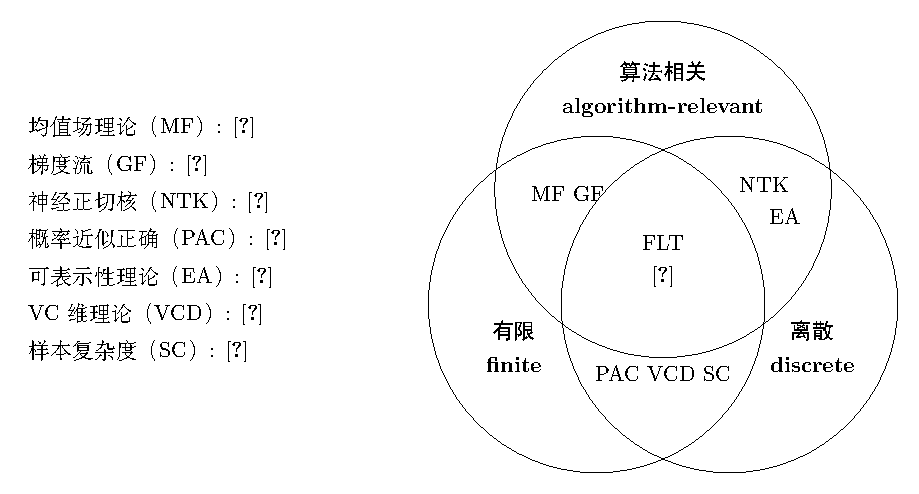
\includegraphics[width=0.99\textwidth]{figures/tikz/learning_theory_taxonomy.pdf}
\else
  \begin{tikzpicture}[scale=1.5]
  % 定义三个圆的中心
  \coordinate (A) at (0,0);
  \coordinate (B) at (1.5,0);
  \coordinate (C) at (0.75,1.3);

  % 画三个圆
  \draw[circle] (A) circle (1.9);
  \draw[circle] (B) circle (1.9);
  \draw[circle] (C) circle (1.9);

  % 标注圆的名称
  \node (finite) at ($(A)+(-0.6,-0.5)$) [above left] {\heiti{有限}};
  \node (finite_ref) at (finite.south) [below] {\textbf{finite}};
  \node (discrete) at ($(B)+(0.6,-0.5)$) [above right] {\heiti{离散}};
  \node (discrete_ref) at (discrete.south) [below] {\textbf{discrete}};
  \node (algorithm_relatedness) at ([yshift=12pt]$(C)+(0,0.7)$) [above] {\heiti{算法相关}};
  \node at (algorithm_relatedness.south) [below] {\textbf{algorithm-relevant}};

  % 圆之间的交集文字
  \node (PAC) at ($(A)!0.5!(B)+(0,-0.6)$) [below] {PAC\ VCD\ SC};
  \node (NTK) at ($(B)!0.5!(C)+(0.4,0.7)$) [right] {NTK};
  \node (EA) at ([xshift=-1pt,yshift=-10pt]NTK) [right] {EA};
  \node at ($(C)!0.5!(A)+(-0.35,0.6)$) [left] {MF\ GF};

  % 三圆交集文字
  \node (FLT) at ($(C)+(0,-0.6)$) {FLT};
  \node (FLT_ref) at (FLT.south) [below] {\cite{DBLP:conf/focs/Allen-ZhuL21}};

  % Caption
  \coordinate (caption1) at ($(A)+(-6.5,2)$);
  \node at (caption1) [right] {均值场理论（MF）: \cite{DBLP:conf/focs/Allen-ZhuL21}};
  \coordinate (caption2) at ([yshift=-12pt]caption1);
  \node at (caption2) [right] {梯度流（GF）: \cite{DBLP:conf/focs/Allen-ZhuL21}};
  \coordinate (caption3) at ([yshift=-12pt]caption2);
  \node at (caption3) [right] {神经正切核（NTK）: \cite{DBLP:conf/focs/Allen-ZhuL21}};
  \coordinate (caption4) at ([yshift=-12pt]caption3);
  \node at (caption4) [right] {概率近似正确（PAC）: \cite{DBLP:conf/focs/Allen-ZhuL21}};
  \coordinate (caption5) at ([yshift=-12pt]caption4);
  \node at (caption5) [right] {可表示性分析（EA）: \cite{DBLP:conf/focs/Allen-ZhuL21}};
  \coordinate (caption6) at ([yshift=-12pt]caption5);
  \node at (caption6) [right] {VC 维理论（VCD）: \cite{DBLP:conf/focs/Allen-ZhuL21}};
  \coordinate (caption7) at ([yshift=-12pt]caption6);
  \node at (caption7) [right] {样本复杂度（SC）: \cite{DBLP:conf/focs/Allen-ZhuL21}};
  \end{tikzpicture}
  \fi

  \caption{机器学习领域主流的理论框架示意图。左：各理论框架常见译名、英文缩写与相关参考文献。右：我们从算法相关性、有限性与离散性三个维度评价各理论框架对于不同学习任务的适用性，以突出FLT与其他理论框架的差异性。如第 \ref{sec-related-works-learning-paradigms} 小节所述，FLT 是一种算法相关、维度有限，且迭代过程离散的理论框架，适用于刻画神经网络的特征学习过程。}
  \label{fig-learning-theory-taxonomy}
\end{figure}

\subsection{FLT的研究进展}
\label{subsec: advance of FLT research}

FLT是一套面向实践应用的理论体系；凡是在实际训练、推理过程中神经网络表现出的性质、现象，都可作为FLT的分析对象与研究载体。
在 FLT 发展初期，研究者主要关注神经网络的一些普遍性质，例如良性过拟合的发生机制\cite{DBLP:conf/nips/0006CBG22}、SGD 算法的优化动力学机理 \cite{DBLP:conf/iclr/LuWYZ24}，以及对比学习（contrastive learning）范式下特征表征的学习机制与优化策略\cite{DBLP:conf/icml/WenL21}等。
在本文的\cref{chap3}，我们分析了对抗训练（adversarial training）的特征学习过程，并聚焦于\emph{特征塌缩}（neural collapse）这一普遍存在于神经网络最后一层特征中的性质。我们将标准训练的结论自然地推广到了对抗训练场景，并量化地分析了特征随对抗训练强度的变化规律及其对模型鲁棒性的影响。

随着与 FLT 相关探索的不断深入，关于神经网络共性的研究已日趋完善。
在此背景下，研究者的关注焦点开始转向更为细分、具体的实践场景或技术环节，例如知识蒸馏的特征迁移机制优化\cite{DBLP:conf/iclr/Allen-ZhuL23}、混合数据增强策略下的特征分布演化规律\cite{DBLP:conf/icml/ZouCLG23}等。
这类研究均旨在从细粒度层面挖掘特征学习的内在机理，为特定技术方案的优化提供理论支撑。
本文\cref{chap4}聚焦重构式异常检测（Reconstruction-Based Anomaly Detection, RBAD）场景下的特征学习动力学过程展开系统分析，最终证实：仅在正常数据上完成训练的生成式网络，在对异常样本进行重构时会产生显著更大的误差，基于这一特性可实现对异常点的有效检测。

随着大语言模型（Large Language Model，LLM）时代到来，关于语言模型（比如TF）与扩散模型（diffusion）的相关问题收到广泛的关注。
% TODO 多CITE一些FLT参考文献
本文基于神经网络研究了QA问题中的知识提取。

综上所述，本文紧跟国内外FLT的研究进展，针对对抗训练、异常检测与机器遗忘这三个学习任务中模型的特征学习机制展开分析。

\section{主要研究问题与技术路线}

在第 \ref{subsec: advance of FLT research} 小节中，我们总结了近几年FLT的研究进展，并
本研究计划围绕特征学习理论的核心科学问题（见\cref{sec-research-questions}），总结现有理论与与相关参考文献，建立统一的分析框架。
随后，我们聚焦对抗训练（adversarial training）、重构式异常检测（reconstruction-based anomaly detection, RBAD）、与LLM问答（question answering, QA）为例，深入考察神经网络在不同任务下的特征提取与演化机制，并总结归纳特征学习的共性特点与不同模型的适配机制。

\subsection{研究问题}\label{sec-research-questions}

本文主要关注下述三个特征学习领域的核心问题。
\begin{mynote}{本文的核心研究问题}
  \begin{itemize}
    \item 特征提取机制：神经网络如何自动从训练数据中提取有效特征？
    \item 特征演化机制：网络提取的特征如何随训练过程演化？
    \item 网络适配机制：为何特定结构的网络只能在一部分学习任务中表现出色？
  \end{itemize}
\end{mynote}
本文将围绕上述三个问题展开研究，并在第六章对每个问题给出简短的回答。

\subsection{技术路线}

\begin{figure}[htbp]
\begin{center}
\iffastcompile
    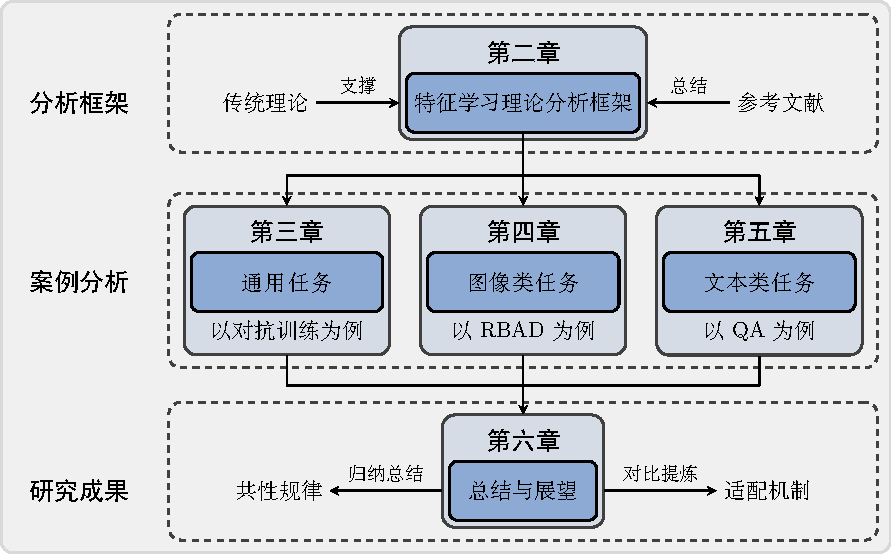
\includegraphics[width=0.99\textwidth]{figures/tikz/research_roadmap.pdf}
\else
    \begin{tikzpicture}[node distance=2cm]
        % 分析框架
        \node (top) [block] {特征学习理论分析框架};
        \node (top_caption) [above] at (top.north) {\zihao{-4}\heiti{第二章}};
        \begin{pgfonlayer}{bg3}
            \node (top_box) [draw=darkgray, fill=blue-background, line width=1pt, rounded corners=6pt, inner sep=0.1cm, fit=(top_caption) (top)] {};
        \end{pgfonlayer}
        \node (theory) [left] at ([xshift=-1.5cm]top.west) {传统理论};
        \node (ref) [right] at ([xshift=1.5cm]top.east) {参考文献};
        \draw [arrow] (theory.east) -- (top_box.west |- theory.east) node [above, midway] {\zihao{-5} 支撑};
        \draw [arrow] (ref.west) -- (top_box.east |- ref.west) node [above, midway] {\zihao{-5} 总结};
        \begin{pgfonlayer}{bg2}
            \node (topbox) [draw=darkgray, dashed, line width=1pt, rounded corners=6pt, inner sep=0.2cm, minimum width=12cm, align=center, fit=(theory) (top_box) (ref)] {};
        \end{pgfonlayer}

        % 案例分析
        \node (mid1) [block, below=of top, xshift=-4cm, text width=3cm] {通用任务};
        \node (mid1_caption) [above] at (mid1.north) {\zihao{-4}\heiti{第三章}};
        \node (mid1_task) [below] at (mid1.south) {以对抗训练为例};
        \begin{pgfonlayer}{bg3}
            \node (mid1_box) [draw=darkgray, fill=blue-background, line width=1pt, rounded corners=6pt, inner sep=0.1cm, fit=(mid1_caption) (mid1) (mid1_task)] {};
        \end{pgfonlayer}
        \node (mid2) [block, below=of top, text width=3cm] {图像类任务};
        \node (mid2_caption) [above] at (mid2.north) {\zihao{-4}\heiti{第四章}};
        \node (mid2_task) [below] at (mid2.south) {以RBAD为例};
        \begin{pgfonlayer}{bg3}
            \node (mid2_box) [draw=darkgray, fill=blue-background, line width=1pt, rounded corners=6pt, inner sep=0.1cm, fit=(mid2_caption) (mid2) (mid2_task)] {};
        \end{pgfonlayer}
        \node (mid3) [block, below=of top, xshift=4cm, text width=3cm] {文本类任务};
        \node (mid3_caption) [above] at (mid3.north) {\zihao{-4}\heiti{第五章}};
        \node (mid3_task) [below] at (mid3.south) {以QA为例};
        \begin{pgfonlayer}{bg3}
            \node (mid3_box) [draw=darkgray, fill=blue-background, line width=1pt, rounded corners=6pt, inner sep=0.1cm, fit=(mid3_caption) (mid3) (mid3_task)] {};
        \end{pgfonlayer}
    
        \begin{pgfonlayer}{bg2}
        \node (midbox) [draw=darkgray, dashed, line width=1pt, rounded corners=6pt, inner sep=0.2cm, minimum width=12cm, align=center, fit=(mid1_box) (mid2_box) (mid3_box)] {};
        \end{pgfonlayer}

        % 研究成果
        \node (bottom) [block, below=2.5cm of mid2] {总结与展望};
        \node (bottom_caption) [above] at (bottom.north) {\zihao{-4}\heiti{第六章}};
        \begin{pgfonlayer}{bg3}
            \node (bottom_box) [draw=darkgray, fill=blue-background, line width=1pt, rounded corners=6pt, inner sep=0.1cm, fit=(bottom_caption) (bottom)] {};
        \end{pgfonlayer}
        \node (modern_theory) [left] at ([xshift=-2cm]bottom.west) {共性规律};
        \node (application) [right] at ([xshift=2cm]bottom.east) {适配机制};
        \draw [arrow] (bottom_box.west |- modern_theory.east) -- (modern_theory.east) node [above, midway] {\zihao{-5} 归纳总结};
        \draw [arrow] (bottom_box.east |- application.west) -- (application.west) node [above, midway] {\zihao{-5} 对比提炼};
        \begin{pgfonlayer}{bg2}
            \node (bottombox) [draw=darkgray, dashed, line width=1pt, rounded corners=6pt, inner sep=0.2cm, minimum width=12cm, align=center, fit=(modern_theory) (bottom_box) (application)] {};
        \end{pgfonlayer}
    
        % 虚线框左上角加标题
        \coordinate (mid_caption) at ($(mid1.west) + (-3cm, 0)$);
        \coordinate (top_caption) at (mid_caption |- theory.west);
        \coordinate (bottom_caption) at (mid_caption |- bottom.west);
        \node (top_summary) [right, inner sep=2pt] at ([xshift=0.2cm]mid_caption) {\zihao{-4}\heiti{案例分析}};
        \node (mid_summary) [right, inner sep=2pt] at ([xshift=0.2cm]top_caption) {\zihao{-4}\heiti{分析框架}};
        \node (bottom_summary) [right, inner sep=2pt] at ([xshift=0.2cm]bottom_caption) {\zihao{-4}\heiti{研究成果}};
    
        % 第一层 -> 第二层
        \coordinate (mid_branch) at ($(mid2_box.north) + (0, 0.5cm)$);
        \coordinate (mid_branch_left) at ($(mid1_box.north) + (0, 0.5cm)$);
        \coordinate (mid_branch_right) at ($(mid3_box.north) + (0, 0.5cm)$);
        \draw [line] (top.south) -- (mid_branch);
        \draw [line] (mid_branch) -- (mid_branch_left);
        \draw [line] (mid_branch) -- (mid_branch_right);
        \draw [arrow] (mid_branch_left) -- (mid1_box.north);
        \draw [arrow] (mid_branch) -- (mid2_box.north);
        \draw [arrow] (mid_branch_right) -- (mid3_box.north);
    
        % 第二层 -> 第三层
        \coordinate (bottom_branch) at ($(mid2_box.south) + (0, -0.5cm)$);
        \coordinate (bottom_branch_left) at ($(mid1_box.south) + (0, -0.5cm)$);
        \coordinate (bottom_branch_right) at ($(mid3_box.south) + (0, -0.5cm)$);
        \draw [line] (mid1_box.south) -- (bottom_branch_left);
        \draw [line] (mid2_box.south) -- (bottom_branch);
        \draw [line] (mid3_box.south) -- (bottom_branch_right);
        \draw [line] (bottom_branch_left) -- (bottom_branch);
        \draw [line] (bottom_branch) -- (bottom_branch_right);
        \draw [arrow] (bottom_branch) -- (bottom_box.north);

        \begin{pgfonlayer}{bg1}
            \node (background) [draw=darkgray-background, fill=darkgray-background!40, line width=1pt, rounded corners=6pt, inner sep=0.2cm, minimum width=0.99\textwidth, align=center, fit=(topbox) (midbox) (bottombox) (mid_caption) (top_caption) (bottom_caption)] {};
        \end{pgfonlayer}
    \end{tikzpicture}
\fi
\end{center}
\end{figure}

\section{本文的主要贡献}

\section{论文结构安排}

本文共有六章，其中\cref{chap1}为绪论，介绍了特征学习理论的研究背景与意义，总结了该领域国内外发展近况，并概括了本文的研究内容与主要贡献。
在\cref{chap2}中，我们结合传统学习理论与现代深度学习的实际应用，总结出了适用于特征学习理论分析的统一分析框架。
在第\ref{chap3}至第\ref{chap5}章中，我们深入探讨了FLT在分析、阐释及优化深度学习实际应用问题中的具体作用与成效。
其中：
\begin{itemize}
  \item 第三章以对抗训练为研究场景，分析全连接神经网络特征学习动力学基础与神经塌缩特性，探究单纯形压缩现象的表征、成因及其与神经塌缩的关联差异，验证其对模型鲁棒性的影响。
  \item 第四章聚焦RBAD场景，探究图像数据与RBAD的适配性，构建卷积神经网络特征学习动力学模型，推导特征提取与数据重建的关联机制并开展实验验证。
  \item 第五章针对问答任务，构建Transformers知识提取动力学模型，解析自注意力机制驱动的知识捕捉与表达逻辑并验证其有效性。第六章对全文研究成果进行总结，分析研究局限性，并展望未来研究方向。
\end{itemize}
本文第\ref{chap3}到第\ref{chap5}章的分析始终围绕着我们在\cref{sec-research-questions}中提到的三个研究问题，即“网络如何自动提取有效特征”、“特征如何随训练过程演化”与“为何特定结构的网络在特定类型的数据上具有更优特征学习能力”。
在第六章，我们总结了全文的核心工作，为上述研究问题提供了一份详细的分析、回答。并就未来的潜在研究方向进行了深入思考。
\chapter{特征学习理论的分析框架}\label{sec-preliminaries}

FLT作为深度学习领域新兴的基础理论分支，既承袭了传统统计学习理论的系统性理论框架，又深受深度学习应用中实际问题的驱动。
本章将从基础定义出发，系统阐述特征学习理论的核心概念与关注焦点。
我们首先基于机器学习理论的视角，解构一般学习任务并剖析其 “四要素”，随后顺势引出“特征”与“特征学习”这两个核心概念，并辅以必要的概率统计工具。
最后，我们将归纳总结特征学习理论的分析框架。

\section{特征学习理论的基本概念}\label{sec-feature-learning-theory-basics}

在本文中，我们分别用小写与大写粗体字母来表示（列）向量和矩阵。
给定$d \in \mathbb{N}^{+}$和$\v \in \R^d$，记$\v$的第$i$个元素（$1 \leq i \leq d$）为$\v^{(i)}$，即$\v = (\v^{(1)}, \v^{(2)}, \cdots, \v^{(d)})^{\top}$。
类似地，我们用$\M^{(i)}$来表示矩阵$\M$的第$i$列，并记$\M = (\M^{(1)}, \M^{(2)}, \cdots, \M^{(d)})$。
给定$N \in \mathbb{N}^{+}$，我们记指标集$\{1, 2, \cdots, N\}$为$[N]$。
对任意$n \in [N]$，为简单起见，我们令$[N \backslash n] := \{ 1, \cdots, n-1, n+1, \cdots, N \}$。

给定模型族$\calF$，机器学习的核心任务是训练一个模型$f \in \calF$，使其能够对输入数据$\z$做出精准的预测。
其中，根据不同的学习任务，$\z$可以取不同的形式，例如图像、文本、基因序列等，而模型的功能则可以是分类、回归、生成或聚类等。
对于任意输入值$\z$，我们可以通过定义一个损失函数（loss function）$\ell(f, \z)$来量化模型预测值$f(\z)$的准确程度。
给定数据集$\calD$，模型$f$在$\calD$上的经验风险（empirical risk）定义为：
\begin{equation}
  \hat{R}(f; \calD) = \frac{1}{|\calD|} \sum_{\z \in \calD} \ell(f, \z).
\end{equation}
经验风险是模型$f$在训练数据集$\calD$上的平均损失，可用于评估模型$f$在训练数据集$\calD$上的性能，并作为优化目标来训练模型。
具体来说，我们希望找到一个模型$f^{*}$，使得经验风险最小化，也即：
\begin{equation}
  f^{*} = \arg \min_{f \in \mathcal{F}} \hat{R}(f; \calD).
\end{equation}
在实际场景中，我们需要借助优化算法来求解上述优化问题。
常见的优化算法包括梯度下降（Gradient Descent，GD）、随机梯度下降（Stochastic Gradient Descent，SGD）、Adam等。
在相关文献中，数据集、模型族、损失函数与优化算法共同定义了一个具体的学习任务，构成了该任务的四大核心要素。

具体来说，我们希望模型$f$能够满足以下条件：
\begin{equation}
  f(\x) = y
\end{equation}
其中$y$是$\x$的标签。
在统计学习理论中，我们通常将模型$f$表示为函数空间$\mathcal{F}$中的一个元素，即$f \in \mathcal{F}$。
我们称$\mathcal{F}$为假设类（hypothesis class）。
我们称$\mathcal{F}$为假设类（hypothesis class）。

学习任务（learning task）一般由数据集、假设类（hypothesis class）、优化算法与评价指标决定。
这四个东西一般也被成为机器学习的四大核心要素。
具体来说，给定数据集$\calD$与假设类$\calH$，我们需要设计一个风险函数$\calR: \calH \times \calD \to \R$来评价模型在学习任务上的性能，
并基于该风险函数设计优化算法$\mathcal{A}$，最终通过评价指标$\mathcal{E}$来评估模型的性能。
数据层面，FLT一般采取信号-噪音模型（Signal-to-Noise Model，SNM）来刻画数据分布。
以图像为例，。
因此，

\begin{proposition}[高维正交性]\label{prop-almost-ortho-in-high-d-space}

\end{proposition}
性质\ref{prop-almost-ortho-in-high-d-space}说明了正交假设的合理性，因为高位空间中的总是趋近于正交的。

\section{特征与特征学学习}\label{sec-feature-and-feature-learning}



\section{特征学习理论的分析框架}\label{sec-feature-learning-theory-analysis-framework}
\chapter{对抗训练的特征学习理论分析}\label{chap-PNAS}

本章将围绕神经网络的特征塌缩 (neural collapse) 现象展开, 并探索其背后的特征学习机制. 
特征塌缩由Papyan等\cite{neural-collapse}首次发现并总结, 是一种普遍存在于神经网络输出层的几何特征. 
具体而言, Papyan等\cite{neural-collapse}研究了分类任务中训练的最终阶段 (Terminal Phase of Training, TPT) , 发现输出层特征在该阶段会坍缩为一个等角紧框架 (Equiangular Tight Frame, ETF) 结构. 


特征塌缩现象已被证实是跨数据集和网络架构的普遍现象. 
许多先前的研究将这一几何结构特征应用于离分布检测\cite{ood}, 长尾学习\cite{longtail}和对抗训练\cite{robnc}等任务. 
本文重点探讨对抗训练 (adversarial training) 下网络的特征学习机制及其在特征塌缩现象中的. 
此处AT指通过特定训练范式增强神经网络对抗鲁棒性的方法\cite{DBLP:journals/corr/GoodfellowSS14}, 具体定义可参阅\ref{sec-at-preliminaries}.
已有研究\cite{robnc}发现, 特征塌缩现象同样存在于对抗训练中.
然而, 通过AT训练的神经网络与传统训练模型存在显著差异\cite{DBLP:conf/nips/VardiYS22,DBLP:conf/nips/FreiVBS23}.
由此引出两个核心问题：
\begin{mynotice}
    \begin{center}
        标准训练与对抗训练的特征学习机制有何本质区别?
    \end{center}
\end{mynotice}
本文的核心目标在于系统阐释标准训练与对抗训练中特征塌缩现象的差异.
具体而言, 我们通过实证研究揭示对抗训练对神经压缩几何结构的影响, 并发现了单纯形压缩现象.
我们在对抗训练的最终阶段, 压缩后的单纯形 ETF 的几何尺寸较标准神经压缩显著缩小, 且随着对抗样本扰动半径的增大, 压缩程度呈现递增趋势.
图\ref{fig-simplex-compression}直观展示了这一研究发现.

我们首先通过实证研究证明, 单纯形压缩现象在各类模型和数据集中普遍存在且具有普适性.
在此基础上, 我们从理论层面阐释了对抗训练引发该现象的作用机制.
我们, 随着扰动半径的增大, 压缩程度会显著增强.
特别值得注意的是, 我们的理论预测与第3.3节展示的实验结果高度吻合, 这为我们的实证发现提供了有力佐证. 

\section{对抗训练与特征塌缩现象的基础概念}\label{sec-nc-preliminaries}

\subsection{对抗训练}\label{sec-at-preliminaries}

先前的研究\cite{DBLP:journals/corr/SzegedyZSBEGF13,trades,wat}表明，对手对输入的细微扰动可能导致神经网络产生错误分类的输出标签，这严重影响了模型的鲁棒性。 
这种被扰动的输入在文献中被称为对抗样本。

许多防御\cite{DBLP:journals/corr/GoodfellowSS14,trades, wat}策略已被开发出来以增强模型对对抗样本的鲁棒性。 
其中，AT作为最有效的防御机制\cite{trades,wat,mart,fat,eat,robnc}出现，它利用精心构造的对抗样本来在训练过程中提高模型的鲁棒性。
具体而言，Madry等\cite{DBLP:conf/iclr/MadryMSTV18}提出了一种开创性的对抗训练方法, 称为投影梯度下降 (\texttt{PGD}) 防御，该方法可以高效地生成对抗训练样本并将其纳入训练阶段。
在PGD之后，涌现出许多改进的对抗训练方法，其中值得注意的例子包括：
\texttt{TRADES} \cite{trades}，它优化了一个平衡鲁棒性与干净准确率的损失函数；以及
\texttt{MART} \cite{mart}，它提出以不同方式处理错误分类和正确分类的样本。
上述方法 (\texttt{PGD-AT}、\texttt{TRADES}和\texttt{MART}) 是研究神经网络对抗鲁棒性的常用基准。
在本文中，我们基于这三种方法探索标准神经网络压缩与对抗神经网络压缩之间的差异。

下面我们引入对抗训练的数学定义.
我们首先引入对抗样本 (adversarial example) 的概念.
在图像分类问题中, 对抗样本$\xa$是一类经过恶意构造的样本, 其在视觉上与干净样本$\x$高度相似, 但会迫使分类器对$\xa$和$\x$做出不同的预测. 
更具体地说, 给定分类器$f$, 对于任意$\x \in \R^d$, 我们称$\xa$为$f$在$\x$处的$\epsilon$-对抗样本, 如果$\xa$满足$f(\x) \neq f(\xa)$且$\|\xa - \x\|_p \leq \epsilon$. 
在此定义中, 常数$\epsilon$量化了$\x$与$\xa$之间允许的最大扰动, 以确保两者的视觉相似性, 在文献中通常被称为 扰动半径 (perturbation radius). 

如上文所述, 对抗训练的核心思想是利用构造出的对抗样本来训练分类器. 
更具体地说, 给定损失函数$\ell$, 对抗训练首先通过最大化$\ell$来生成对抗样本, 即
\begin{equation}\label{eq:advsample}
\xa_{k,n} := \mathop{\argmax}_{\x \in B_\epsilon(\x_{k,n})} \ell\left(f\left( \x \right), y_{k}\right),
\end{equation}
其中$B_\epsilon(\x_{k,n}) := \{ \x : \|\x - \x_{k,n}  \|_p  \leq \epsilon \}$是围绕$\x_{k,n}$的关于$p$-范数的$\epsilon$-球.
基于公式\ref{eq:advsample}中的定义, 对抗训练随后最小化以下经验对抗训练风险:
\begin{equation}
\begin{aligned}
\label{eq-def-adversarial-risk}
    \Radv(f,\mathcal{D})
   :&= \frac{1}{NK} \sum_{(\x_{k,n},y_k) \in \mathcal{D}} \ell\left(f\left( \xa_{k,n} \right), y_{k}\right) \\
    &= \frac{1}{NK} \sum_{(\x_{k,n},y_k) \in \mathcal{D}} \max_{\x \in B_\epsilon(\x_{k,n})} \ell\left(f\left( \x \right), y_{k}\right).
\end{aligned}
\end{equation}
得到的分类器记为$f^* = \argmin_f \Radv(f, \mathcal{D})$.

\subsection{特征塌缩}\label{sec-neural-collapse-setup}

在\ref{sec-feature-and-feature-learning} 中, 我们引入了特征提取器的概念：一个神经网络分类器通常由一个特征提取器 (feature extractor) 和一个线性分类器 (linear classifier) 组合而成. 
在本文中, 我们用$\boldsymbol{h}: \R^d \to \R^{\dpr}$来表示特征提取器. 
对于任意输入$\x \in \R^d$, $\h(\x)$在文献中通常被称为最后一层特征 (last layer feature) , 也即\ref{sec-feature-and-feature-learning} 中所提到的高级特征. 
这里, $d^{\prime}$表示最后一层特征的维度. 
特征塌缩现象主要涵盖了以下四个特征：

\begin{definition}[特征塌缩]\label{def-neural-collapse}
    给定特征提取器$\boldsymbol{h}: \R^d \to \R^{\dpr}$, 我们称$\h$发生了特征塌缩现象, 如果$\h$满足以下四个性质 (记为\textbf{(NC1)} - \textbf{(NC4)}):
    \begin{itemize}
        \item \textbf{(NC1)} {\heiti 方差塌缩}: 
            通过计算单个类别$k$中所有特征的平均值, 我们可以得到第$k$类的类均值向量 ($k$-th class mean vector) 
            \begin{equation}\label{eq-def-class-mean-vector}
            \boldsymbol{\bar{h}}_{k} := \frac{1}{N} \sum_{n\in [N]} \h(\x_{k,n}).
            \end{equation}
            方差塌缩指的是在TPT阶段, 最后一层特征的类内方差趋于$0$, 即：
            \begin{equation}
            \left\|  \boldsymbol{\bar{h} } _{k} - \h(\x_{k,n}) \right\|_{2}  \to 0 , \quad \forall  k \in [K], n \in [N].
            \end{equation}

        \item \textbf{(NC2)} {\heiti 收敛到广义单纯形等角紧框架}: 在TPT阶段, 最后一层特征的类均值向量收敛到定义\ref{def-simplex-ETF}给出的广义单纯形ETF. 
        为了便于实证验证, Papyan等\cite{neural-collapse}进一步引入了以下数值特征来刻画\textbf{(NC2)}
            \begin{equation}\label{eq-def-equiv-converge-to-simplex-ETF}
                \begin{aligned}
                &\left | \left \| \boldsymbol{\bar{h} } _{k} - \boldsymbol{\bar{h} } _{G} \right \|_{2} - \left \| \boldsymbol{\bar{h} } _{k^{\prime} } - \boldsymbol{\bar{h} } _{G} \right \|_{2} \right | \to 0, \quad \forall k \neq k^{\prime},\\
                &\cos \left ( \boldsymbol{\bar{h} } _{k}- \boldsymbol{\bar{h} } _{G}, \boldsymbol{\bar{h} } _{k^{\prime}} - \boldsymbol{\bar{h} } _{G}\right )\to-\frac{1}{K-1}  , \quad \forall k\ne k^{\prime},
                \end{aligned}
            \end{equation}
        其中$\boldsymbol{\bar{h}}_{G} := \frac{1}{K} \sum_{k=1}^{K}\boldsymbol{\bar{h} }_{k}$被成为中心化类均值向量 (centralized class mean vector). 
        公式\ref{eq-def-equiv-converge-to-simplex-ETF}表明中心化类均值向量将收敛到一个单纯形ETF.
 
        \item \textbf{(NC3)} {\heiti 收敛到自对偶性}在TPT阶段, 类均值向量和线性分类器收敛到彼此的重新缩放版本, 即：
        \begin{equation}
        \left\|\frac{\boldsymbol{W}^{\top}}{\|\boldsymbol{W}\|_{F}}-\frac{\dot{\boldsymbol{M}}}{\|\dot{\boldsymbol{M}}\|_{F}}\right\|_{F} \rightarrow 0 ,
        \end{equation}
        其中 $\dot{\boldsymbol{M}} = \left(\boldsymbol{\bar{h}}_{1}-\boldsymbol{\bar{h}}_{G}, \boldsymbol{\bar{h}}_{2}-\boldsymbol{\bar{h}}_{G}, \cdots, \boldsymbol{\bar{h}}_{K}-\boldsymbol{\bar{h}}_{G} \right) \in \mathbb{R}^{d^{\prime} \times k}$ 被成为中心化类均值矩阵 (centralized class mean matrix).

        \item \textbf{(NC4)} {\heiti 退化到$k$-近邻算法}:
        在TPT阶段, 分类器会趋近于选择与训练类均值最近 (在标准欧氏距离下) 的类别, 即：
            \begin{equation}
            \arg \max _{k^{\prime}}\left\langle\boldsymbol{w}_{k^{\prime}}, \boldsymbol{h}\right\rangle+b_{k^{\prime}} \rightarrow \underset{k^{\prime}}{\arg \min }\left\|\boldsymbol{h}-\boldsymbol{\bar{h}}_{k^{\prime}}\right\|_{2}.
            \end{equation}
        其中 $\tilde{\boldsymbol{\mu}}_{c}=\left(\boldsymbol{\mu}_{c}-\boldsymbol{\mu}_{G}\right) /\left\|\boldsymbol{\mu}_{c}-\boldsymbol{\mu}_{G}\right\|_{2}$ 为重新缩放地类均值 (renormalized class mean). 
    \end{itemize}
\end{definition}

特征压缩现象刻画了神经网络特征提取器的几何特征. 
许多研究已经证明, 多种不同场景下, 不同网络在不同数据集上都观测到了定义\ref{def-neural-collapse}中所描述的四个特性, 说明NC是神经网络的TPT阶段会出现的一个普遍现象. 
在这四个特征中, \textbf{(NC2)}是最相关的, 因为它揭示了标准和对抗特征塌缩之间最显著的区别, 即广义单纯形ETF定义的单纯形压缩现象. 
因此, 本文的剩余部分将主要关注\textbf{(NC2)}. 

\begin{definition}[广义单纯形等角紧框架\cite{neural-collapse}]
  \label{def-simplex-ETF}
  给定正整数 $d^{\prime} > K$与矩阵
  \begin{equation}
      \W = (\W_1, \W_2, \cdots, \W_K) \in \R^{\dpr \times K}
  \end{equation}
  如果$\W = c_1 \boldsymbol{U} \boldsymbol{M} $成立, 则我们称$\W$为一个广义单纯形等角紧框架. 
  其中
  \begin{equation}\label{eq-def-simplex-ETF-M}
      \boldsymbol{M} 
      = \sqrt{\frac{K}{K-1}} 
      \left( \boldsymbol{I}_{K} -\frac{1}{K} \mathbf{1}_{K}  \mathbf{1}_{K}^{\top}  \right) \in \R^{K \times K},
  \end{equation}
  $\boldsymbol{U}\in \mathbb{R} ^{d^{\prime}\times K }$ 是一个半正交矩阵 (partial orthogonal matrix) , 即$\boldsymbol{U^{\top } }\boldsymbol{U} =\boldsymbol{I}$, 且$c_1 \in \R$是一个非零常数. 
  
  \end{definition}
  值得指出的是, 在NC研究中, 单纯形ETF的定义与数学文献中的定义略有不同 \cite{arXiv:math/0301135,arXiv:1504.00253}. 
  为了消除歧义, 本文中所有关于单纯形ETF的讨论都基于定义\ref{def-simplex-ETF}. 

\section{实证研究}\label{sec-nc-experiment}
本章将通过实证研究, 系统地探索标准和对抗特征塌缩之间的差异. 
我们首先研究对抗特征塌缩现象, 然后探索对抗特征塌缩与标准特征塌缩之间的差异, 揭示单纯形压缩现象. 
我们还提供了一系列消融实验, 以消除扰动范数和PGD迭代步数的影响. 

\subsection{实验设置}\label{sec-nc-experiment-setup}

\paragraph{数据集}我们使用以下三个视觉数据集进行实验. 
\texttt{CIFAR-10} \cite{cifar10} 包含 60,000 张 32x32 像素的彩色图像, 分为 10 类, 每类 6,000 张. 
\texttt{CIFAR-100} 包含 60,000 张 32x32 像素的彩色图像, 分为 100 类, 每类 600 张. 
\texttt{Tiny ImageNet} \cite{deng2009imagenet} 包含 200 类, 每类 500 张 64x64 像素的彩色图像. 

\paragraph{模型} 我们使用\texttt{VGG} \cite{simonyan2014very}, \texttt{ResNet-18} \cite{he2016deep}, 和Wide ResNet (\texttt{WRN}) \cite{wrn} 进行实验. 
具体的选择网络深度和宽度取决于数据集. 
我们参考支持信息文件获取更多细节. 
 
\paragraph{对抗训练方法} 我们使用三种基于PGD的对抗训练方法, 包括标准\texttt{PGD-AT} \cite{DBLP:conf/iclr/MadryMSTV18}, \texttt{TRADES} \cite{trades}, 和\texttt{MART} \cite{mart}. 
许多之前的工作 \cite{robnc, wat, eat} 使用这些方法作为基准. 许多之前的工作 \cite{robnc, wat, eat} 使用这些方法作为基准. 
我们设置PGD的最大迭代步数为 $T_{a}=\left \{ 10,20,30 \right \} $, 扰动半径为 $\epsilon=\left \{2/255, 4/255,  6/255, 8/255\right \} $ 用于 $L_{\infty}$ 范数, 和 $\epsilon=\left \{0.125, 0.250, 0.375, 0.500\right \} $ 用于 $L_2$ 范数. 
我们的 $T_a$ 和 $\epsilon$ 的选择与许多之前的工作 \cite{fat,mart,trades,eat,DBLP:conf/icml/WangPDL0Y23} 和社区的标准化对抗鲁棒性基准\footnote{\href{https://robustbench.github.io/}{https://robustbench.github.io/}} 一致. 

\paragraph{实现细节}我们在Ubuntu 64位Linux工作站上使用PyTorch \cite{pytorch} 实现实验, 该工作站配备10核Intel Xeon Silver CPU (2.20 GHz) 和8个Nvidia GeForce RTX 4090 GPU. 所有网络都训练200个epoch以达到训练的TPT阶段, 此时特征塌缩现象发生. 我们使用动量=0.9和权重衰减=0.001的随机梯度下降 (SGD) . 批量大小为128, 学习率为0.001. 我们保持其他参数与参考文献 \cite{fat,trades,mart,DBLP:conf/iclr/MadryMSTV18} 一致. 

%%%%%%%%%%%%%%%%%%%%%%%%%%%%%%%%%%%% Empirical Exploration-Neural Collapse %  %%%%%%%%%%%%%%%%%%

\subsection{对抗训练中的特征塌缩现象}\label{sec-Empirical Exploration-Neural Collapse}
在节中, 我们训练\texttt{ResNet-18}在\texttt{CIFAR-10}数据集上使用\texttt{PGD-AT}, \texttt{MART}和\texttt{TRADES}. 
对于每个epoch, 我们使用对抗样本计算NC1-NC4的数值特征. 
如图\ref{fig:Neural Collapse}所示, 我们的实验证实了在设置中发生了NC现象 (NC1-NC4) , 从而为我们提供了分析的基础. 
这个观察与之前研究 \cite{robnc,neural-collapse} 的发现一致. 
剩余的结果可以在支持信息文件中找到 (参见图S2 - S10) . 

\begin{figure}[H]
    \centering
    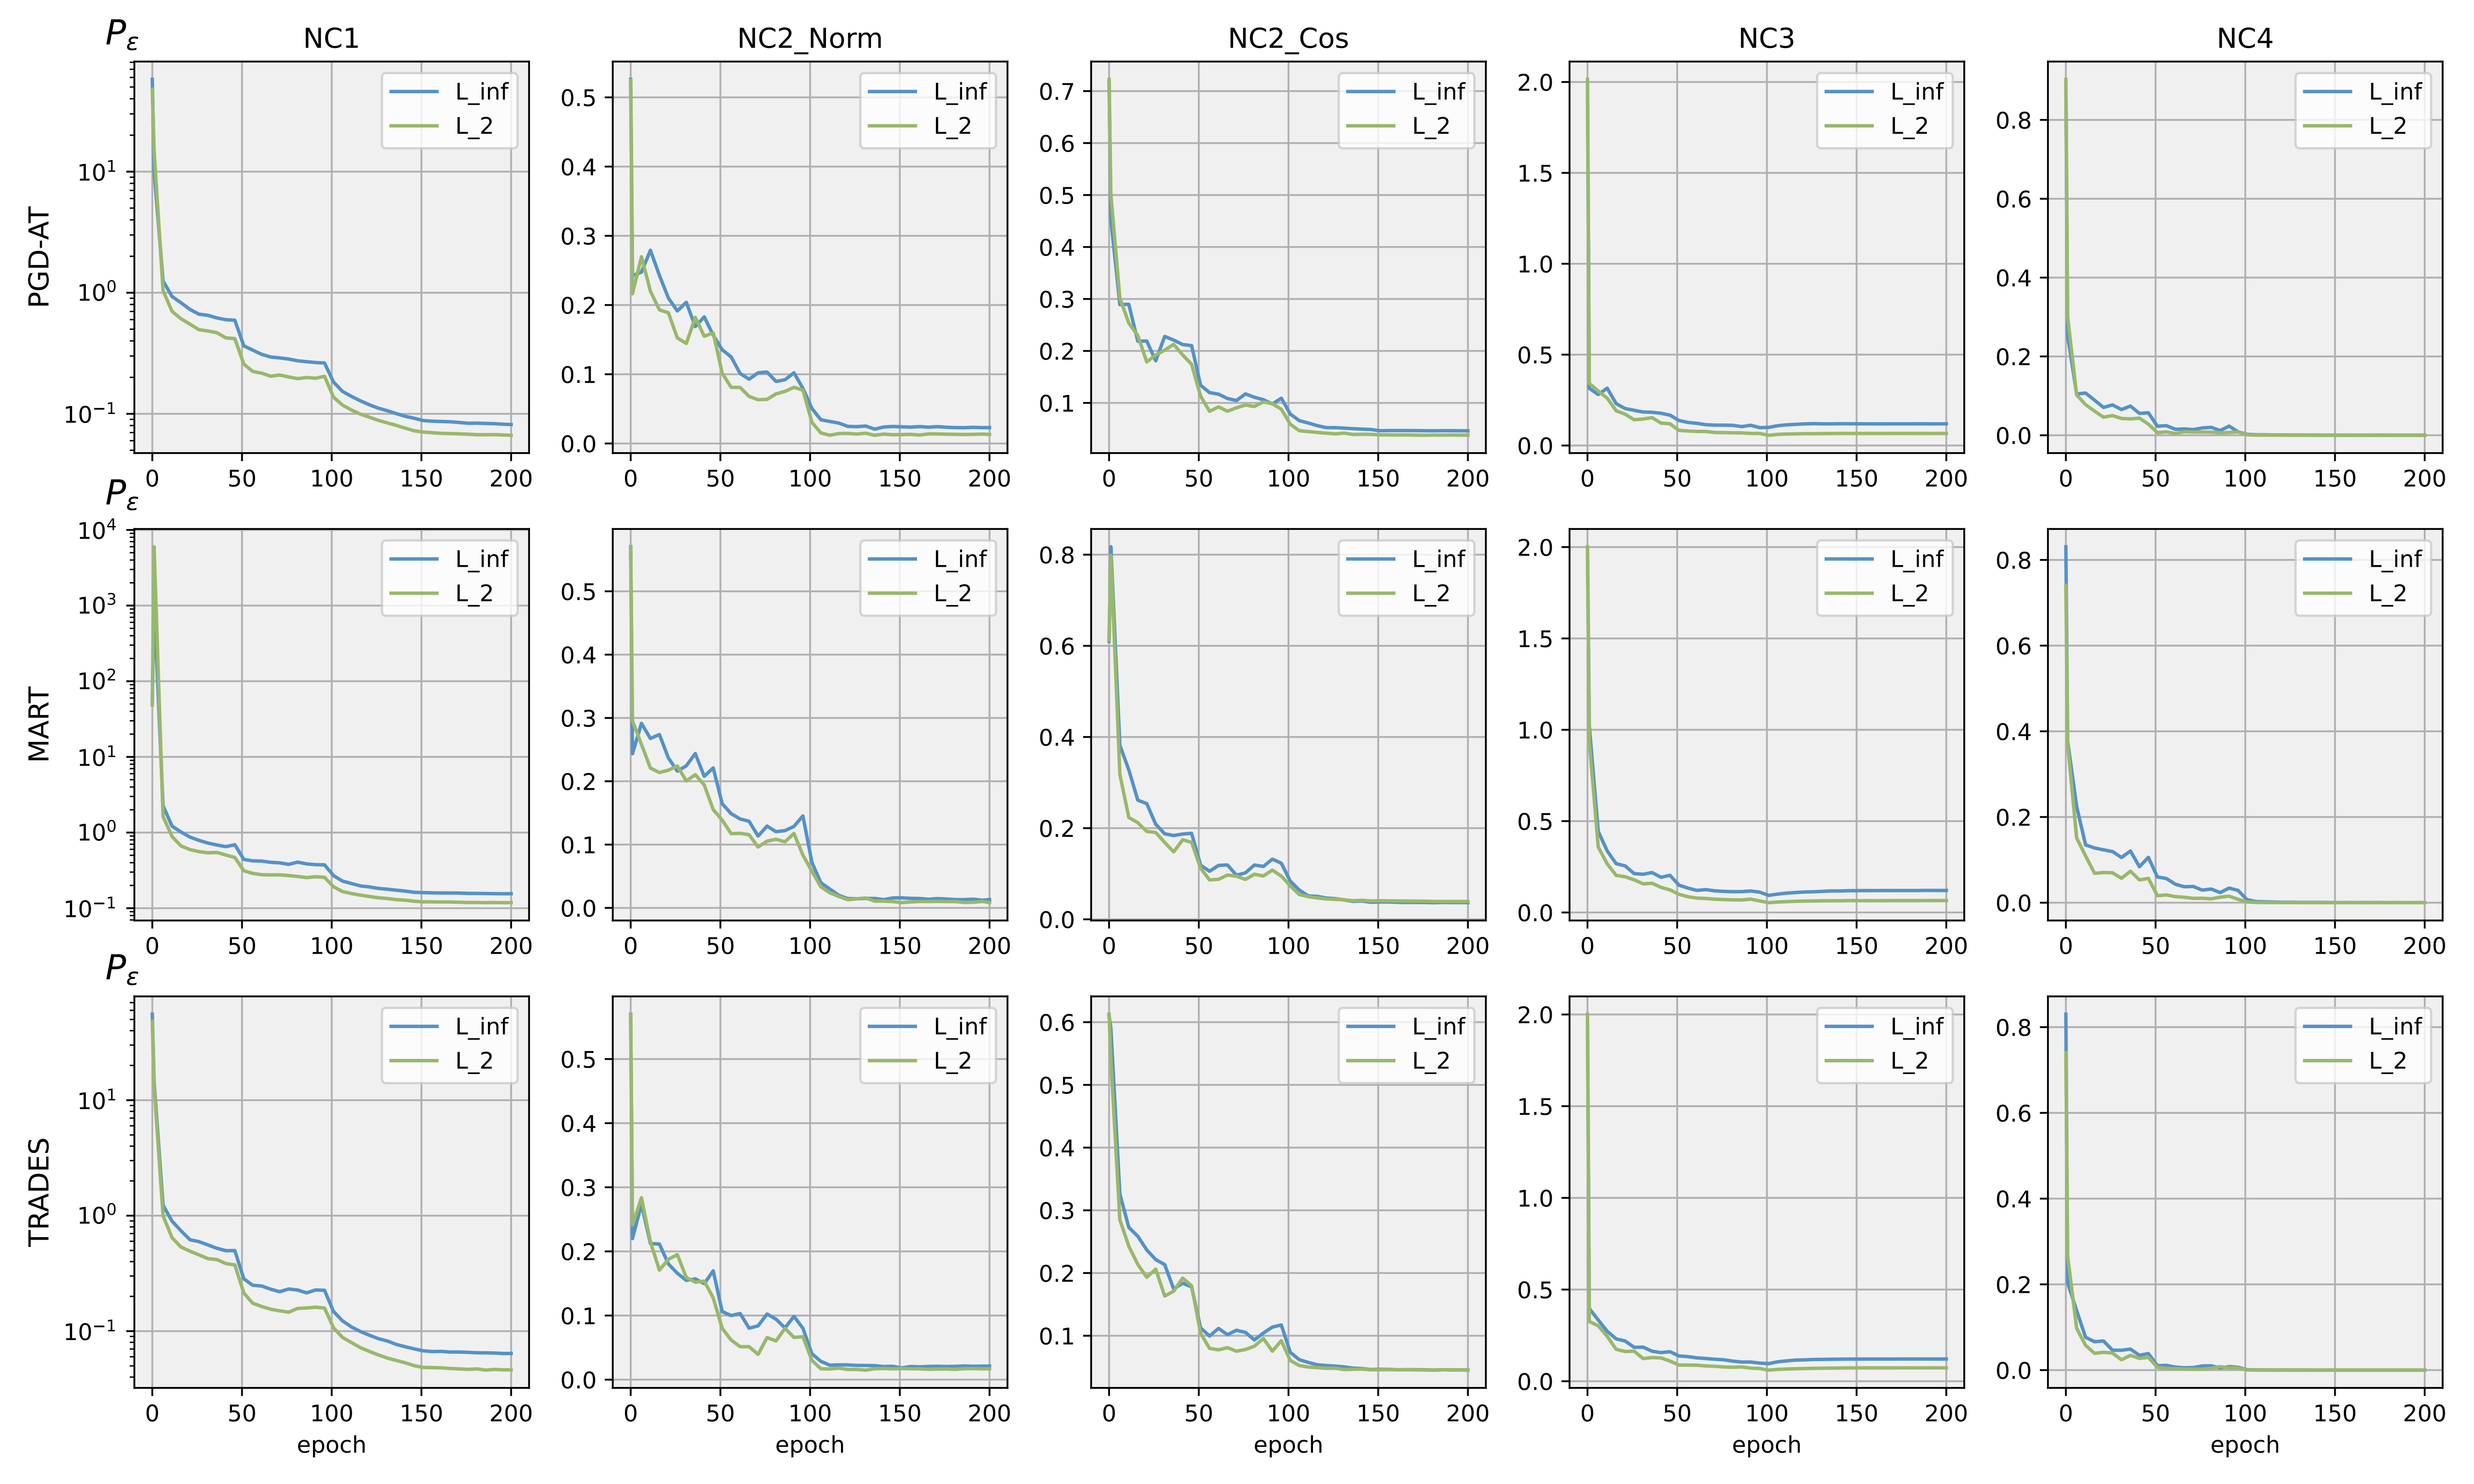
\includegraphics[width=1\linewidth]{figures/nc_main/nc-1.png}
    \caption{
      结果为$NC1,NC2\_Norm,NC2\_Cos,NC3,NC4$. 
      我们在\texttt{CIFAR-10}数据集上使用\texttt{PGD-AT}, \texttt{MART}和\texttt{TRADES}训练\texttt{ResNet-18}. 
      扰动半径设置为$\epsilon=8/255$用于$L_\infty $($L_{\infty} $)和$\epsilon=0.125$用于$L_2$. 
      我们设置$T_{a}=10$.
      结果来自对抗样本.
      }
    \label{fig:Neural Collapse}
\end{figure}

  %%%%%%%%%%%%%%%%%%%%%%%%   Empirical Exploration-Simplex Collapse Phenomenon  %%%%%%%%%%%%%%%%%%%%%%%%%%%%%%%%%%%
\subsection{单纯形压缩现象}\label{sec-simplex-compression-phenomenon}
本节中, 我们考察对抗训练对最后一层特征表示的影响. 
我们定义类间特征距离的平均值为每个类均值向量与全局均值向量之间的差异, 数学表达为：
\begin{equation}\label{eq-def-P-eps}
\boldsymbol{P}_{\epsilon} = \frac{1}{K} \sum_{k=1}^{K} \left \|  \boldsymbol{\bar{h}}_{k} - \boldsymbol{\bar{h}}_{G}  \right \|_{2}.
\end{equation}
我们设置相同的扰动半径$\epsilon$和PGD迭代步数进行实验. 
结果如图\ref{fig-simplex-compression}所示 ($L_2$范数的实验结果见附录图S1) . 
我们可以看到, 随着扰动半径的增加, $\boldsymbol{P}_{\epsilon}$减小. 
这个观察表明单纯形ETF结构的几何尺寸随着扰动半径的增加而减小. 
我们称这种塌缩ETF压缩的现象为单纯形压缩现象. 
单纯形压缩现象的解释是, 对抗训练得到的类均值向量比干净训练得到的类均值向量更相似. 
单纯形压缩现象可以被视为模型鲁棒性的一种特征. 

\subsection{消融实验}\label{sec-Ablation Experiment}
% \subsection{Ablation Experiment}\label{sec-Ablation Experiment}

在 AT 中, 超参数的选择对模型的鲁棒性和适应性至关重要. 
具体来说, 选择量化对抗样本和自然样本之间差异的范数是关键. 
$L_\infty$范数关注扰动向量的最大分量, $L_2$范数测量干净样本和对抗样本之间的欧氏距离. 
两者都是常用的范数来刻画对抗扰动. 
此外, 生成对抗样本的迭代过程, 如等式\eqref{eq:advsample}所示, 需要多次迭代才能收敛. 

% In the context of AT, the selection of hyper-parameters plays a pivotal role in defining the robustness and adaptability of learning models. 
% Specifically, the choice of norms to quantify the deviation between adversarial and natural examples is critical. 
% The $L_\infty$ norm focuses on the maximum component of the perturbation vector, and the $L_2$ norm measures the Euclidean distance between clean examples and adversarial examples.
% Both are commonly used norms for characterizing adversarial perturbations.
% Furthermore, the iterative process of generating adversarial examples, as delineated in Equation \eqref{eq:advsample}, necessitates multiple iterations for convergence. 

为了研究超参数对单纯形压缩现象的影响, 我们设计了消融实验. 
我们设置PGD迭代步数为$T_{a}=\left \{10, 20 ,30\right \} $, 扰动半径为$\epsilon=\left\{0,2/255,4/255,6/255,8/255\right\}$用于$L_\infty$范数, 和$\epsilon=\left\{0,0.125,0.250,0.375,0.500\right\}$用于$L_2$范数. 
结果如图 \ref{fig:pgd_effect} 所示. 
我们可以看到, 单纯形压缩现象在不同的PGD迭代步数和扰动半径下都存在. 


% To investigate the potential confounding effects of these hyper-parameters in previous experiments, we design additional experiments with varying hyperparameter selections. 
% For the $L_\infty$ norm, perturbation radius are set to $\epsilon=\left\{0,2/255,4/255,6/255,8/255\right\}$, while for the $L_2$ norm, they are adjusted to $\epsilon=\left\{0,0.125,0.250,0.375,0.500\right\}$. 
% These selections are consistent with those used in previous experiments. And we set PGD iterations $T_{a}=\left \{10, 20 ,30\right \} $ to repeat our experiments.
% The results are displayed in \ref{fig:pgd_effect}. 
% We can see that simplex compression exits for different perturbation norms and PGD iterations.

此外, 我们通过展示干净样本的$\boldsymbol{P}_{\epsilon}$结果, 进一步扩展了我们的分析. 
如图\ref{fig-sample-effect}所示, 我们观察到干净样本的$\boldsymbol{P}_{\epsilon}$值相对于对抗样本较大, 但它们与单纯形压缩现象保持一致. 

\section{关于单纯形压缩现象的理论解释}\label{sec-theoretical-explanation}

在本节中, 我们通过分析干净训练和对抗训练过程, 理论解释单纯形压缩现象. 
我们指定数据模型, 网络结构和训练范式在\ref{sec-nc-preliminaries}中. 
假设总结在\ref{subsec-nc-assumptions}中. 
我们将在\ref{subsec-theoretical-main-results}中展示主要结果, 并将证明推迟到支持信息文件中. 

\subsection{符号}\label{subsec-notations}
我们在\ref{sec-feature-learning-theory-basics}中引入了一些符号. 
在本节中, 我们重述一些关键符号以保持完整性. 
给定$K \in \mathbb{Z}^+$, 我们的分析专注于具有$K$个类的平衡分类任务. 
后续段落详细描述了数据模型, 网络结构和训练范式. 

\paragraph{数据模型}
在我们的论文中, 样本被收集在配备欧几里得范数$\|\cdot\|$的欧几里得空间$\R^d$上. 
我们记$[K]:= \{ 1,2, \cdots, K \}$为方便. 
对于任意$\x_1, \x_2 \in \R^{d}$, $\x_1$和$\x_2$的内积 (点积) 记为$\x_1^{\top}\x_2$. 
给定$N \in \mathbb{Z}^+$, 平衡训练数据集$\mathcal{D}$有$N$个样本, 每个类一个, 记为
\begin{equation}\label{eq-def-dataset}
    \mathcal{D} :=  \{  (\x_{k, n} ,y_{k}) :  k \in [K], n \in [N] \},    
\end{equation}
其中$\x_{k,n} \in \R^d$和$y_k \in [K]$分别是训练样本和其标签. 
我们还使用$y(\x)$来表示$\x$的标签, 当它不明确时. 
向量 (列) 的元素记为
\begin{equation}
    \x = (\x^{(1)}, \x^{(2)}, \cdots, \x^{(d)})^{\top}.    
\end{equation}

\paragraph{网络结构}
在分类任务中, 一个基于神经网络的分类器$f$被用来将样本映射到每个类的预测概率. 
以前的研究倾向于使用UFM来表征$f$. 
下面的注释指出了原始UFM的一个局限性. 

\begin{remark}[UFM的局限性]\label{remark-ufm}
    UFM将最后一层特征$\h$视为独立的可优化变量. 
    然而, 我们的研究需要控制对$\x$应用小扰动后$\h$的变化 (即引入对抗样本) . 
    因此, 将$\h$视为独立变量可能不适合分析对抗训练下的特征塌缩现象. 
    
\end{remark}

在本文中, 我们采用以下方式表征$f$：
\begin{definition}[$f$的表征]\label{def-f}
令$f: \R^d \to \R^K$为一个2层神经网络分类器, 定义为：
\begin{itemize}
    \item 给定$\x \in \R^d$, $f$的第一层是一个特征提取器$\h$, 记为$\h(\x) = {\relu}( \w^{\top} \x + \bbeta) \in \R^{d^{\prime}}$, 它将输入样本$\x$映射到特征$\h(\x)$. 
    \item $f$的第二层是一个线性分类器, 记为$\softmax(\W^{\top} \h(\x) + \b) \in \R^K$, 它将特征映射到预测概率. 
\end{itemize}
得到的分类器记为
\begin{equation}
\begin{aligned}
    f(\x)
    &= \softmax(\W^{\top} \h(\x) + \b) \\
    &= \softmax(\W^{\top} \left( {\relu}( \w^{\top} \x + \boldsymbol{\beta}) \right) + \b)
\end{aligned}
\end{equation}
对于任意$\x \in \R^d$. 

\end{definition}

我们提供以下解释来介绍\ref{def-f}中引入的新术语. 
$d^{\prime} \in \mathbb{Z}^{+}$是最后一层的维度. 
$\bbeta \in \R^{\dpr}$和$\b \in \R^k$是向量；
$\w \in \R^{d \times \dpr}$和$\W \in \R^{\dpr \times K}$是矩阵. 
$\softmax(\cdot)$用于归一化输出概率, 定义为
\begin{equation}\label{eq-def-softmax}
  \softmax(\u)^{(i)} = \frac{\exp(\u^{(i)})}{\sum_{j \in [K]}(\exp(\u^{(j)}))}
\end{equation}
对于任意$\u \in \R^K$. 
$\relu(\cdot)$定义为
\begin{equation}
  \relu(u) = \left\{
  \begin{aligned}
      0,& \ {\rm{if}}\ u \in [0, \theta] \\
      u,& \ {\rm{if}}\ u \notin [0,\theta]
  \end{aligned}
  \right.
\end{equation}
对于任意$u \in \R$和给定参数$\theta > 0$. 
下面这条注释讨论了以前工作中用于描述特征$\h(\x)$的各种术语. 

\begin{remark}
  特征$\h(\x)$位于NC分析的中心部分, 可以被视为最后一层和倒数第二层的输入和输出. 
  因此,  ``最后一层特征'' 和 ``倒数第二层特征'' 在NC的上下文中通常指的是同一个概念. 
  
\end{remark}

\paragraph{训练范式}
我们首先介绍干净训练的范式. 
干净训练的损失函数定义为
\begin{equation}
  \ell(f(\x), y(\x)) = - \log \left( f(\x)^{(y(\x))} \right).
\end{equation}
然后, 干净训练的风险定义为
\begin{equation}
  R(f,\mathcal{D}) := \frac{1}{NK} \sum_{(\x, y(\x)) \in \mathcal{D}} \ell(f(\x), y(\x)).
\end{equation}
给定正步长$\eta$, 特征提取器$\h$根据以下梯度下降规则更新：
\begin{equation}
  \h^{\iter{t+1}} = \h^{\iter{t}} - \eta \nabla_{\h^{\iter{t}}} R(f, \mathcal{D}).
\end{equation}
在第$t$次迭代时. 

我们接着介绍对抗训练的范式. 
我们采取投影梯度下降的策略来生成对抗样本. 
回忆\ref{eq-def-adversarial-risk}中定义的对抗风险为
\begin{equation}
\label{eq-def-adversarial-risk-restate}
    \Radv(f,\mathcal{D})
    = \frac{1}{NK} \sum_{(\x_{k,n},y_k) \in \mathcal{D}} \ell\left(f\left( \xa_{k,n} \right), y_{k}\right),
\end{equation}
其中对抗样本是通过有限步投影梯度下降生成的. 
更具体地说, 给定干净样本$\x$和最大PGD步数$T_a$, 对抗样本$\xa$的生成规则为

\begin{equation}\label{eq-def-gradient-based-attack-itertion}
\begin{aligned}
    \x^{0} &= \x, \\
    \x^{\tau+1} &= \x^{\tau} + \epsilon \nabla_{\x^{\tau}} \ell(f(\x^{\tau}), y(\x^{\tau})),
\end{aligned}
\end{equation}
对于任意 $0 \leq \tau < T_a$.
对抗训练涉及对每个$\x_{k,n} \in \mathcal{D}$生成对抗样本, 可以表示为
\begin{equation}\label{eq-def-gradient-based-attack}
    \xa_{k,n} = \x_{k, n} + \sum_{t \in [T_a] } \epsilon \nabla_{\x^{\tau}_{k,n}} \ell(f(\x^{\tau}_{k,n}), y_k).  
\end{equation}
其中$\epsilon$是扰动半径, 用于重缩放对抗攻击.
值得注意的是, 当$\epsilon=0$时, 对抗训练退化为干净训练. 

对抗训练的迭代规则为
\begin{equation}\label{eq-def-GD-AT}
    \h^{\iter{t+1}} = \h^{\iter{t}} - \eta \nabla_{\h^{\iter{t}}} \Radv(f, \mathcal{D}).
\end{equation}
注意, 我们还没有指定公式\ref{eq-def-GD-AT}和\ref{eq-def-GD}中迭代的初始化设定.

\subsection{理论分析假设}\label{subsec-nc-assumptions}
本节介绍了一系列必要假设, 用于分析NC在AT下的行为, 包括归一化, TPT和NC3假设.

\paragraph{归一化} 由于NC的几何性质在实证观察中需要适当的重缩放与中心化, 我们也采用如下归一化假设：

\begin{itemize}
    \item 训练数据是对称的, 即我们假设
    \begin{equation}
        \left\{
    \begin{aligned}
        (\w_{l}^{\iter{T_0}})^{\top} \x_{k,n} \geq \theta,& \ {\rm{if}}\ l = k \\
        (\w_{l}^{\iter{T_0}})^{\top} \x_{k,n} \leq 0,& \ {\rm{if}}\ l \neq k
    \end{aligned}
    \right.
    \end{equation}
    我们推迟$T_0$的定义到\ref{assumption-tpt}.
    \item 同一类内的相似性和不同类之间的差异被归一化. 
    具体来说, 给定$\rho > 0$, 对于所有$n_1, n_2 \in [N]$和$k_1 \neq k_2 \in [K]$, 我们假设
    \begin{enumerate}
        \item $(\x_{k,n_1})^{\top} \x_{k,n_2} \in [1-\rho,1+\rho]$, for all $n_1, n_2 \in [N]$,
        \item $(\x_{k_1,n_1})^{\top} \x_{k_2,n_2} \in [-\rho, \rho]$, for all $k_1 \neq k_2 \in [K]$. 
    \end{enumerate}
    注意到$\rho$和$K$是独立的.
    \item $f$的偏置项被设定为$0$, 此即我们假设在中心化后有$\bbeta = \0$, 且在选择一个合适的变换后有$\b = \0$.
\end{itemize}


{\vspace{0.5em}\noindent{\heiti{TBT}}\hspace{0.5em}}
如\ref{sec-nc-preliminaries}所述, 标准和对抗NC都发生在TPT期间.
这里, TPT指的是训练风险收敛到接近零之后的训练轮次.
根据定义, 我们有
\begin{equation}\label{eq-exp-loss-function}
    \exp(\ell(f(\x_{k,n}),y_k)) = \frac{\sum_{k^{\prime}} \exp \left( \W^{\top}_{k^{\prime}} \h(\x_{k,n}) \right)}{\exp \left( \W^{\top}_k \h(\x_{k,n}) \right)}.
\end{equation}
利用公式ref{eq-exp-loss-function}, 我们可以如下刻画TPT.
\begin{assumption}[TPT]\label{assumption-tpt}
在本文的剩余部分, 训练终止阶段 (Terminal Phase of Training, TPT) 被刻画如下.
对于所有$k \in [K]$, $l \neq k$, 和$n \in [N]$, 我们用$T_0$表示TPT的起始步.
我们假设$T_0$具备如下性质:
\begin{equation}\label{eq-def-assumption-TPT-k}
    \frac{\exp \left( \W^{\top}_k \h^{\{T_0\}}(\x_{k,n}) \right)}
    {\sum_{k^{\prime}} \exp \left( \W^{\top}_{k^{\prime}} \h^{\{T_0\}}(\x_{k,n}) \right)} = 1 - \sigma
\end{equation}
以及
\begin{equation}\label{eq-def-assumption-TPT-k1-k2}
    \frac{\exp \left( \W^{\top}_{l} \h^{\{T_0\}}(\x_{k,n}) \right)}
    {\sum_{k^{\prime}} \exp \left( \W^{\top}_{k^{\prime}} \h^{\{T_0\}}(\x_{k,n}) \right)} = \frac{\sigma}{K-1}.
\end{equation}
在公式\ref{eq-def-assumption-TPT-k}和\ref{eq-def-assumption-TPT-k1-k2}中, 参数$\sigma \in (0, 1)$用于刻画训练的精度.
值得注意的是, 如果$\sigma=0$, 训练风险变为零.
 
\end{assumption}

以下推论可以直接由\ref{assumption-tpt}推出.
\begin{corollary}\label{corollary-TPT}
    设$C_1 > C_2 > 0$为参数. 
    如果我们对所有$k \in [K]$, $l \neq k$, $n \in [N]$和$i \in \{1, 2\}$令$\W_k \h^{\iter{t_i}}(\x_{k,n}) = C_i$和$\W_{l} \h^{\iter{t_i}}(\x_{k,n}) = -C_{i} (K-1)^{-1}$, 那么 
    \begin{equation*}
        \frac{\exp \left( \W^{\top}_k \h^{\{t_1\}}(\x_{k,n}) \right)}
        {\sum_{k^{\prime}} \exp \left( \W^{\top}_{k^{\prime}} \h^{\{t_1\}}(\x_{k,n}) \right)} 
        > 
        \frac{\exp \left( \W^{\top}_k \h^{\{t_2\}}(\x_{k,n}) \right)}
        {\sum_{k^{\prime}} \exp \left( \W^{\top}_{k^{\prime}} \h^{\{t_2\}}(\x_{k,n}) \right)}.
    \end{equation*}
\end{corollary}

值得注意的是, 对所有$k \in [K]$, $n \in [N]$, 和$l \neq k$有$\W_k \h(\x_{k,n}) = C$和$\W_{l} \h(\x_{k,n}) = -C (K-1)^{-1}$意味着$\h$收敛到单纯形ETF (归一化后).
在这个意义上, \ref{corollary-TPT}表明特征更好地收敛到单纯形ETF并不意味着更小的训练误差.

为了便于更准确地比较标准和对抗NC, 我们假设干净训练和AT的迭代都从\( T_0 \)开始, 即我们在公式\ref{eq-def-GD-AT}和\ref{eq-def-GD}中要求\( t \geq T_0 \).


\paragraph{NC3} 
由于我们分析的主要焦点集中在NC2和$\h$上, 为简单起见, 我们假设NC3中关于$\W$的结果在TPT开始时成立.
更具体地说, 我们基于\ref{def-simplex-ETF}采用以下假设.
\begin{assumption}[NC3]\label{assumption-NC3}
我们假设线性分类器$\W$在TPT开始时已收敛到单纯形ETF.
具体地, 设$\boldsymbol{M}$表示\ref{eq-def-simplex-ETF-M}中定义的矩阵, 我们假设
\begin{equation}
    \W = c_1 \boldsymbol{U} \boldsymbol{M} = \sqrt{\frac{K-1}{K}} \left( \boldsymbol{e}_1, \boldsymbol{e}_2, \cdots, \boldsymbol{e}_K  \right) \boldsymbol{M},
\end{equation}
其中$\left( \boldsymbol{e}_1, \boldsymbol{e}_2, \cdots, \boldsymbol{e}_K  \right) \in \R^{\dpr \times K}$是一个二元半正交矩阵, 使得对于任意$k \in [K]$, 只有$\boldsymbol{e}_k$的第$k$个元素取$1$, 而其他元素取$0$. 
\end{assumption}

注意到取$c_1 = \sqrt{\frac{K-1}{K}}$和$\boldsymbol{U} = \left( \boldsymbol{e}_1, \boldsymbol{e}_2, \cdots, \boldsymbol{e}_K  \right)$不失一般性, 因为单纯形ETF在正交变换下是不变的. 


\subsection{主要结论}\label{subsec-theoretical-main-results}
对于任意$k \in [K]$和$t \geq T_0$, 设
\begin{equation}
    \boldsymbol{\bar{h}}^{\iter{t}}_{k} := \frac{1}{N} \sum_{n\in [N]} \h^{\iter{t}}(\x_{k,n})
\end{equation}
为第$t$次迭代时的第$k$类均值向量 (参见\ref{eq-def-class-mean-vector}).
我们首先在假设\ref{subsec-nc-assumptions}中的假设下验证NC2.

\begin{theorem}[NC2]\label{theorem-NC2}
给定扰动半径$\epsilon$, 存在常数$\boldsymbol{P}_{0},\boldsymbol{P}_{\epsilon} \in \R$使得在干净训练当中, 类均值向量满足
\begin{equation}
    \bar{\h}^{(k)}_k \to \boldsymbol{P}_{0} (K-1){K}^{-1}, \bar{\h}^{(l)}_k \to -\boldsymbol{P}_{0} K^{-1},
\end{equation}
且在对抗训练当中, 满足
\begin{equation}
    \bar{\h}^{(k)}_k \to \boldsymbol{P}_{\epsilon} (K-1){K}^{-1}, \bar{\h}^{(l)}_k \to -\boldsymbol{P}_{\epsilon} K^{-1}
\end{equation}
对所有$k \in [K]$和$l \neq K$成立, 当$t \to \infty$和$\rho \to 0$时.
\end{theorem}

定理\ref{theorem-NC2}表明类均值向量在干净训练和AT中都收敛到单纯形ETF, 这验证了我们关于NC2的实证结果.
$\boldsymbol{P}_{0}$和$\boldsymbol{P}_{\epsilon}$的几何解释是\ref{eq-def-P-eps}中的单纯形范数 (相差一个缩放因子).
此外, 我们可以基于\ref{theorem-NC2}证明以下结果.
\begin{theorem}[单纯形压缩]\label{theorem-simplex-compression}
设$\boldsymbol{P}_{0},\boldsymbol{P}_{\epsilon} \in \R$为\ref{theorem-NC2}中指定的常数.
我们可以证明当$\epsilon=0$时, 有
\begin{equation}
    \boldsymbol{P}_{0} = \boldsymbol{P}_{\epsilon},
\end{equation}
且对任意$\epsilon_1 > \epsilon_2 \geq 0$, 有
\begin{equation}
    \boldsymbol{P}_{\epsilon_1} < \boldsymbol{P}_{\epsilon_2}.
\end{equation}
\end{theorem}
定理\ref{theorem-simplex-compression}证明了扰动半径 ($\epsilon$) 与单纯形范数 ($\boldsymbol{P}_{0}, \boldsymbol{P}_{\epsilon}$) 之间的负相关关系, 这进一步验证了单纯形压缩现象.

我们分析的核心直觉参见图\ref{fig-intuition}.
给定$k \in [K]$, 我们证明$\boldsymbol{h}(\x_{k,n})$沿着由$\W_k$决定的主方向比其他方向表现出更快的增长率. 
随着训练迭代的进行, $\boldsymbol{h}(\x)$会逐渐更紧密地与单纯形ETF结构对齐. 
更重要的是, 我们证明了训练数据中对抗样本的存在会削弱来自$\x$的信号, 从而降低$\boldsymbol{h}(\x)$的增长率, 从而引发单纯形压缩现象.

\begin{figure}[H]
  \centering
  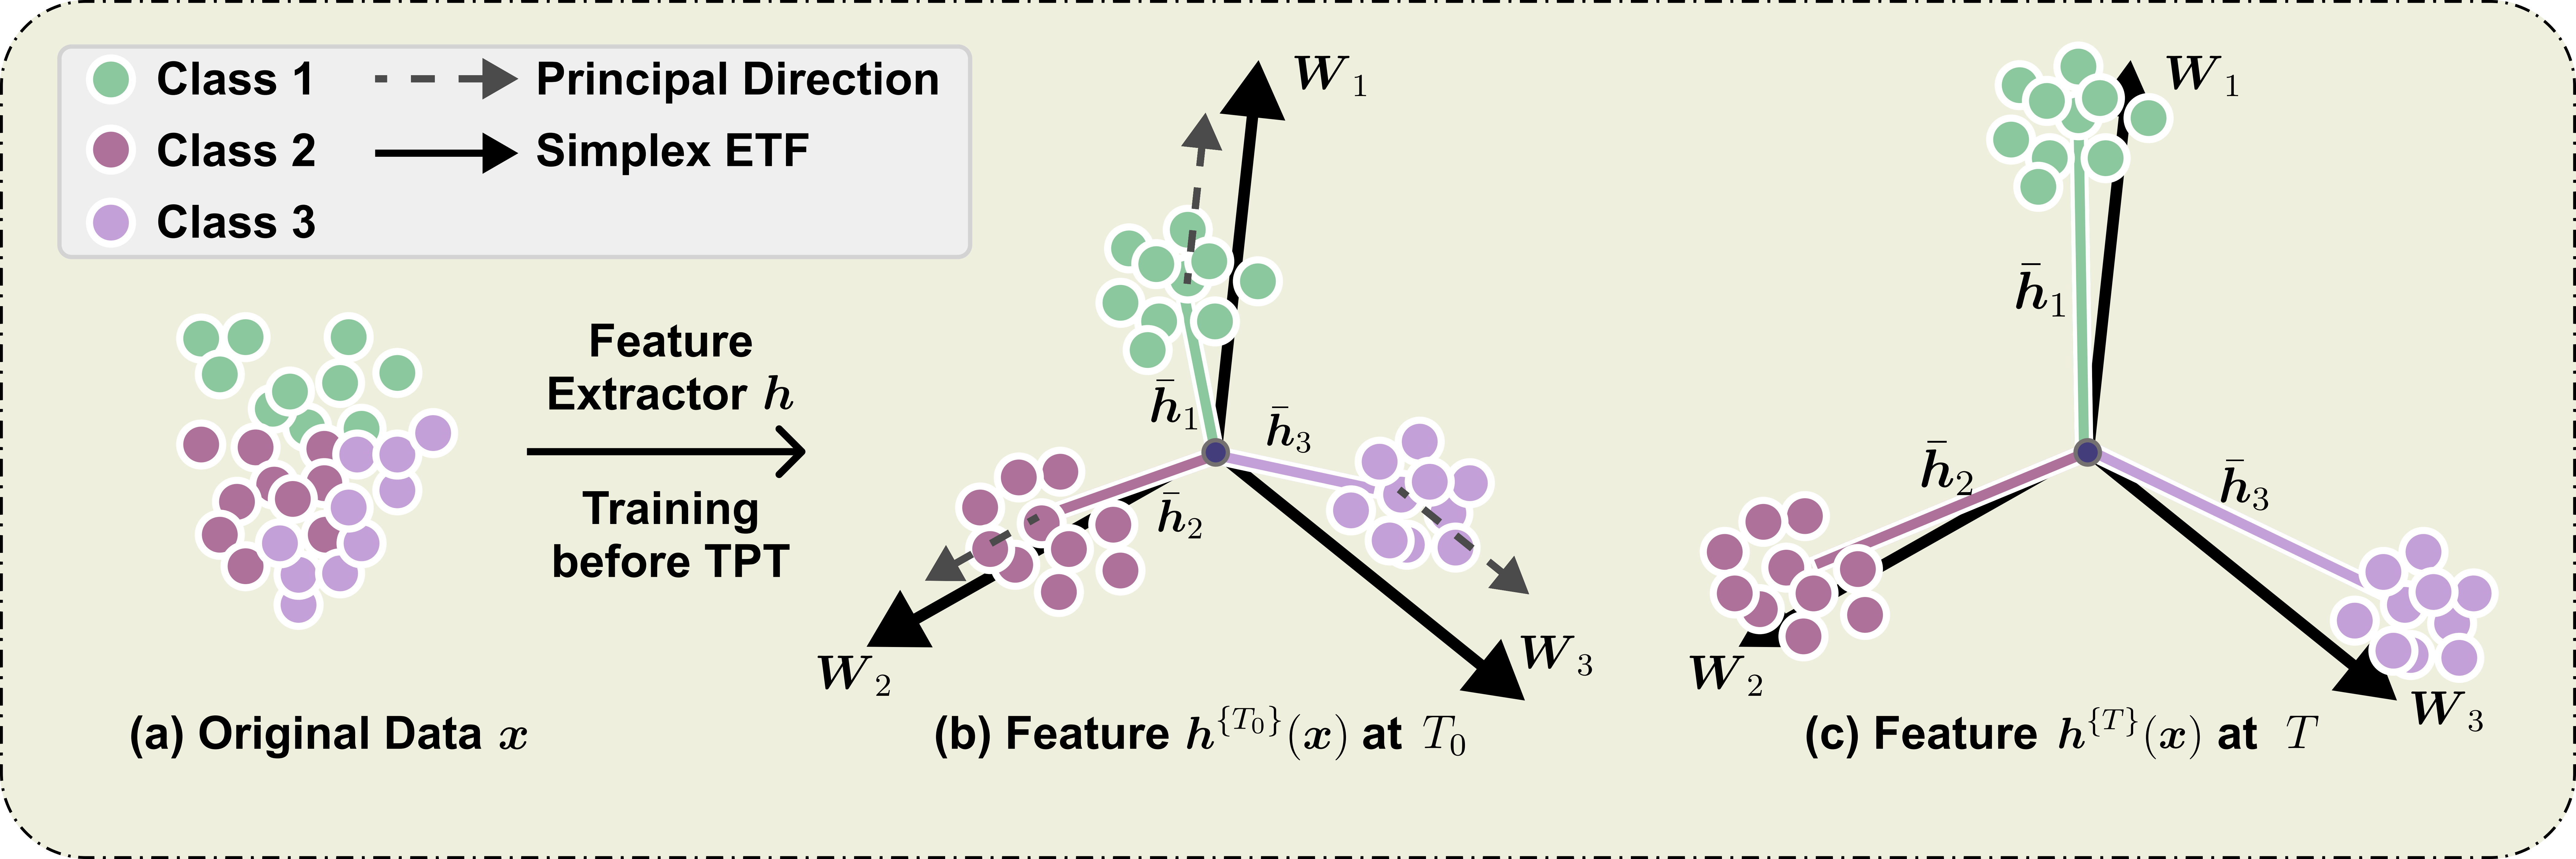
\includegraphics[width=\textwidth]{figures/nc_main/intuition.png}
  \caption{我们理论分析核心直觉的图示. 为了便于可视化, 我们考虑一个$2$维空间中的$3$类分类任务. }
  \label{fig-intuition}
\end{figure}

\subsection{主要结论证明}\label{subsec-main-proof}

我们分析的主要目标可以总结如下.
\begin{mynotice}
    \textit{
    我们的目标是证明存在$C, C^{adv} \in \R$使得
    \begin{itemize}
        \item 在干净训练下, 对所有$k \in [K]$和$l \neq k$有$\w_k \x_{k,n} \to C (K-1){K}^{-1}$和$\w_{l} \x_{k,n} \to -C (K)^{-1}$ (\ref{lemma-TPT-clean}), 且
        \item 在AT下, 对所有$k \in [K]$和$l \neq k$有$\w_k \x_{k,n} \to C^{adv} (K-1){K}^{-1}$和$\w_{l} \x_{k,n} \to -C^{adv} (K)^{-1}$ (\ref{lemma-TPT-AT}).
    \end{itemize}
    更重要的是, 我们证明$C > C^{adv}$, 这说明了单纯形压缩现象.
    我们还证明了扰动半径$\epsilon$与压缩率之间的正相关关系.
    }
\end{mynotice}

证明概要可以总结如下. 
\begin{mynotice}
    \begin{itemize}
        \item \textit{定理\ref{theorem-NC2}和\ref{theorem-simplex-compression}可以由引理\ref{lemma-TPT-AT}与\ref{lemma-TPT-clean}一同推出.}
        \item \textit{引理\ref{lemma-principal-entry-of-h}可以直接由假设\ref{assumption-tpt}和\ref{assumption-NC3}推导得出.}
        \item \textit{引理\ref{lemma-TPT-AT}和\ref{lemma-TPT-clean}的证明主要使用了数学归纳法.}
    \end{itemize}
\end{mynotice}

首先, 我们先回顾并介绍一些技术细节.
回顾我们在公式\ref{eq-def-dataset}中定义的平衡训练数据集$\mathcal{D}$，其中每个类别有$N$个样本，记为
\begin{equation}
    \mathcal{D} :=  \{  (\x_{k, n} ,y_{k}) :  k \in [K], n \in [N] \},    
\end{equation}
其中$\x_{k,n} \in \R^d$和$y_k \in [K]$分别是训练样本及其标签。
我们也用$(\x, y(\x)) \in \mathcal{D}$表示训练数据集中的非特定标记样本。
一个基于两层神经网络的分类器$f: \R^d \to \R^{K}$由下式给出
\begin{equation}\label{eq-def-UFM}
    f(\x) = f(\x; \W, \h, \b) = \softmax(\W^{\top} \h(\x) + \b) \in \R^K,
\end{equation}
其中softmax函数的定义由公式\ref{eq-def-softmax}给出.
矩阵$\W = (\W_1, \W_2, \cdots, \W_K) \in \R^{\dpr \times K}$和向量$\b=(b_1, b_2, \cdots, b_K)^{\top} \in \R^K$分别是最后一层的权重和偏置项，其中$\dpr$是该层的宽度。
$\h: \R^d \to \R^{\dpr}$是将样本映射到最后一层特征的\textit{特征提取器}。

干净训练和对抗训练的范式重述如下。
$f$的干净训练遵循标准的\textit{经验风险最小化}范式，其\textit{交叉熵损失}定义为
\begin{equation}\label{eq-def-loss-function}
\begin{aligned}
    \ell(f(\x_{k,n}), y_k)
    &= - \log \left( \softmax\left(\W^{\top} \h(\x_{k,n}) + \b\right)^{(k)} \right) \\
    &= - \left( \W_k^{\top} \h(\x_{k,n}) + b_k \right) + \log \sum_{j \in [K]}  \exp\left( \W_j^{\top} \h(\x_{j,n}) + b_j \right).
\end{aligned}
\end{equation}
为简化记号，我们将$f$的线性层输出（即$\softmax$函数的输入）简化为
\begin{equation}\label{eq-def-o}
    \o(\x_{k,n}) := \W^{\top} \h(\x_{k,n}) + \b   \nonumber 
    = \left(\W_1^{\top} \h(\x_{k,n}) + b_1, \cdots, \W_K^{\top} \h(\x_{k,n}) +  b_K\right)^{\top}.
\end{equation}
在证明的其余部分，我们也将用$\o_{k,n} \equiv \o(\x_{k,n})$表示。
使用公式\ref{eq-def-o}中的记号, \textit{经验风险}可以写为
\begin{equation}\label{eq-def-clean-risk-with-specified-loss-function}
  R(\W, \h, \b) := \frac{1}{NK} \sum_{k \in [K]} \sum_{n \in [N]} \ell(f(\x_{k,n}), y_k)
   = \frac{1}{NK} \sum_{k \in [K]} \sum_{n \in [N]} \left(\log \sum_{j \in [K]} \exp\left({\o^{(j)}_{k,n}}\right) - \o^{(k)}_{k,n} \right).
\end{equation}
在本文的主要部分，我们记\( R = R(f, \mathcal{D}) \)，这本质上等价于\( R = R(\boldsymbol{W}, \boldsymbol{h}, \boldsymbol{b}) \)。 
在整个证明中，这两种记号可以互换使用。
为了获得优化的特征提取器，我们求解以下优化问题
\begin{equation}\label{eq-def-optimization-problem}
    \h^{\ast} = \mathop{\argmin}_{\h} R(\W, \h, \b).
\end{equation}
对于所有$t \geq 0$，$\h$的梯度下降迭代规则由下式给出
\begin{equation}\label{eq-def-GD-h}
    \h^{\iter{t+1}} = \h^{\iter{t}} - \eta \nabla_{\h^{\iter{t}}} R(\W, \h, \b).
\end{equation}
在公式\ref{eq-def-GD-h}中，$\nabla_{\h} R(\W, \h, \b)$表示经验风险关于$\h$的梯度，由以下引理给出。

\begin{lemma}\label{lemma-nabla-h-R-Whb}
经验风险关于$\h$的梯度可以写为
\begin{equation}\label{eq-nabla-h-final-in-lemma}
  \nabla_{\h} R(\W, \h, \b) = \frac{1}{NK} \sum_{k \in [K]} \sum_{n \in [N]} \left( \sum_{k^{\prime} \in [K]}
  \left( \frac{\exp \left(\o^{(k^{\prime})}(\x_{k,n})\right)}{\sum_{j \in [K]} \exp\left(\o^{(j)}(\x_{k,n})\right)} - \delta_{k^{\prime}k} \right) \W_{k^{\prime}} \right) .
\end{equation}
\end{lemma}

\begin{proof}[引理\ref{lemma-nabla-h-R-Whb}]
根据定义，我们有
\begin{equation}\label{eq-def-nabla-h}
    \nabla_{\h} R(\W, \h, \b) 
    = 
    \frac{1}{NK} \sum_{k \in [K]} \sum_{n \in [N]}
    \nabla_{\h} \left(  \log \sum_{j \in [K]} 
        \exp\left({\o^{(j)}_{k,n}}\right) - \o^{(k)}_{k,n} 
    \right).
\end{equation}
这里，对于任意$k \in K$和$n \in N$，我们有
\begin{equation}\label{eq-def-nabla-h-1}
    \nabla_{\h} \left( \log \sum_{j \in [K]}
    \exp\left({\o^{(j)}_{k,n}}\right) - \o^{(k)}_{k,n}  
    \right) 
  = J_{\o_{k,n}} (\h)        
    \nabla_{\o_{k,n}} \left( \log \sum_{j \in [K]}
        \exp\left({\o^{(j)}_{k,n}}\right) - \o^{(k)}_{k,n}  
    \right)
\end{equation}
在公式\ref{eq-def-nabla-h-1}中，$J_{\o_{k,n}} (\h)$表示（转置的）雅可比矩阵。
根据定义，我们可以得到
\begin{equation}\label{def-eq-jacobian-h-W}
    J_{\o_{k,n}} (\h)
    := \left( \nabla_{\h} \o_{k,n}^{(1)}, \nabla_{\h} \o_{k,n}^{(2)}, \cdots, \nabla_{\h} \o_{k,n}^{(K)}  \right) = \W.
\end{equation}
除了$J_{\o_{k,n}} (\h)$之外，公式\ref{eq-def-nabla-h-1}右侧的另一项可以简化如下。 
对于所有$k^{\prime} \in [K]$，我们有
\begin{equation}\label{eq-def-nabla-o-jprime-x-kn}
    \nabla_{{\o}^{(k^{\prime})}_{k,n}} 
    \left(\log \sum_{j \in [K]}
        \exp\left({\o^{(j)}_{k,n}}\right) - \o^{(k)}_{k,n} 
    \right)
    = \frac{\exp \left(
        \o^{(k^{\prime})}_{k,n}
    \right)}
    {\sum_{j \in [K]} \exp(\o^{(j)}_{k,n})} - \delta_{k^{\prime}k}.
\end{equation}
这里，$\delta_{k^{\prime}k}$是一个二元函数，当$k^{\prime} = k$时取值为$1$，否则为$0$。
结合公式\ref{eq-def-nabla-h-1},公式\ref{def-eq-jacobian-h-W}和公式\ref{eq-def-nabla-o-jprime-x-kn}，我们有
\begin{equation}
    \nabla_{\h} \left( \log \sum_{j \in [K]}
    \exp\left({\o^{(j)}_{k,n}}\right) - \o^{(k)}_{k,n}  
    \right)
    = \sum_{k^{\prime} \in [K]} \left( \frac{\exp \left(\o^{(k^{\prime})(\x_{k,n})}\right)}{\sum_{j \in [K]} \exp\left(\o^{(j)}(\x_{k,n})\right)} - \delta_{k^{\prime}k} \right) \W_{k^{\prime}},
\end{equation}
最终我们可以将$\nabla_{\h} R(\W, \h, \b)$简化为
\begin{equation}\label{eq-nabla-h-final}
  \nabla_{\h} R(\W, \h, \b) = \frac{1}{NK} \sum_{k \in [K]} \sum_{n \in [N]} \left( \sum_{k^{\prime} \in [K]}
  \left( \frac{\exp \left(\o^{(k^{\prime})}(\x_{k,n})\right)}{\sum_{j \in [K]} \exp\left(\o^{(j)}(\x_{k,n})\right)} - \delta_{k^{\prime}k} \right) \W_{k^{\prime}} \right) .
\end{equation}
这完成了证明。
值得注意的是，公式\ref{eq-def-nabla-h-1}中$J_{\o_{k,n}} (\h) = \W$的矩阵乘法在公式\ref{eq-nabla-h-final}中被重新表述为对列向量$\W_{k^{\prime}}$的求和。
\end{proof}

对抗训练需要关于$\x$的梯度信息来构造用于训练的对抗样本。
更具体地说，对于任意$\x \in \R^d$，损失函数的梯度为
\begin{equation}\label{eq-nabla-x-l}
    \nabla_{\x} \ell(f(\x), y(\x)) 
    = \sum_{l \in [K]} \ell^{\prime}_l (f(\x), y(\x)) \nabla_{\x} \o^{(l)}
    = \sum_{l \in [K]} \ell^{\prime}_l (\x, y(\x)) \left(\nabla_{\x} \h(\x)\right)^{\top} \W_l . 
\end{equation}
这里，稍微滥用记号，我们记
\begin{equation}\label{eq-def-ell-prime}
    \ell^{\prime}_l (\x_{k,n}, y_k) 
   := \frac{\partial}{\partial \o^{(l)}_{k,n}} \ell(f(\x_{k,n}), y_k) 
   = \frac{\exp\left( \o_{k,n}^{(l)} \right) }{\sum_{j \in [K]} \exp \left( \o^{(j)}_{k,n} \right) } - \delta_{lk}.
\end{equation}

公式\ref{eq-nabla-x-l}中项$\nabla_{\x} \h(\x)$的分析需要关于$\h$的函数性质的额外假设。
我们将在后续章节中重新讨论这一关键方面。
基于梯度的对抗攻击（例如，类似PGD的攻击）以最多$T_a$步通过迭代以下规则生成对抗样本
\begin{equation}
\begin{aligned}
    \x^{0} &= \x, \\
    \x^{\tau+1} &= \x^{\tau} + \epsilon \nabla_{\x^{\tau}} \ell(f(\x^{\tau}), y(\x^{\tau})), \quad 0 \leq \tau \leq T_a.
\end{aligned}
\end{equation}
对抗训练涉及为每个$\x_{k,n} \in \mathcal{D}$生成对抗样本，这可以表征为
\begin{equation}
    \xa_{k,n} = \x_{k, n} + \sum_{t \in [T_a] } \epsilon \nabla_{\x^{\tau}_{k,n}} \ell(f(\x^{\tau}_{k,n}), y_k).  
\end{equation}

结合上述方程，我们可以将\textit{对抗风险}指定为
\begin{equation}
\label{eq-adversarial-risk-specific}
\Radv(\W, \h, \b)
=  \frac{1}{NK} \sum_{k \in [K]} \sum_{n \in [N]} \ell\left(f\left( \xa_{k,n} \right), y_{k}\right).
\end{equation}
与干净训练相比，对抗训练过程稍微复杂一些。
如\cite{fat}所建议的，在对抗训练开始阶段引入过于强大的对抗样本可能会阻止神经网络学习干净特征。
因此，我们考虑以下两阶段建模用于对抗训练。
更具体地说，对于任意$j \in [\dpr]$，我们让对抗训练的迭代规则在前$T_0$次迭代中与干净训练相同（参见公式\ref{eq-def-GD-h}）。对于所有$t \geq T_0$，我们通过以下方式指定对抗训练的迭代规则
\begin{equation}
\h^{\iter{t+1}} = \h^{\iter{t}} - \eta \nabla_{\h^{\iter{t}}} \Radv(\W, \h, \b) 
\end{equation}
换句话说，我们只在终端阶段（TPT）考虑对抗训练。 
由于我们理论分析的主要目标是解释单纯形压缩现象的原因，我们认为终端阶段之前的迭代步骤并不重要，因为神经网络压缩（NC）只发生在终端阶段。
以下推论直接来自公式\ref{lemma-nabla-h-R-Whb}，它计算对抗风险的梯度。

\begin{corollary}\label{corollary-nabla-h-Radv-Whb}
对抗风险关于$\h$的梯度为
\begin{equation}\label{eq-nabla-h-Radv-final-in-corollary}
  \nabla_{\h} \Radv(\W, \h, \b) = \frac{1}{NK} \sum_{k \in [K]} \sum_{n \in [N]} \left( \sum_{k^{\prime} \in [K]}
  \left( \frac{\exp \left(\o^{(k^{\prime})}(\x^{adv}_{k,n})\right)}{\sum_{j \in [K]} \exp(\o^{(j)}(\x^{adv}_{k,n}))} - \delta_{k^{\prime}k} \right) \W_{k^{\prime}} \right) .
\end{equation}
\end{corollary}
\begin{proof}[推论\ref{corollary-nabla-h-Radv-Whb}]
    该推论直接由公式\ref{lemma-nabla-h-R-Whb}得出。
\end{proof}

设$\relu(\cdot)$为
\begin{equation}\label{eq-def-relu}
    \relu(u) = \left\{
    \begin{aligned}
        0,& \ {\rm{if}}\ u \in [0, \theta] \\
        u,& \ {\rm{if}}\ u \notin [0,\theta]
    \end{aligned}
    \right.
\end{equation}
对于任意$u \in \R$和某个给定的$\theta > 0$。
稍微滥用记号，我们将$\relu$激活函数按元素扩展到向量和矩阵，并考虑以下特征提取器

\begin{equation}\label{eq-def-feature-extractor}
    \h(\x) = \relu( \w^{\top} \x + \bbeta),
\end{equation}
其中$\w = (\w_1, \w_2, \cdots, \w_{\dpr}) \in \R^{K \times \dpr}$是$\h$的权重，$\bbeta = (\beta_1, \beta_2, \cdots, \beta_{d^{\prime}})$是偏置项。
对于任意$\x \in \R^d$和$i,l \in [\dpr]$，$\h(\x)$的项及其导数\footnote{严格来说，$\relu$在$u = \pm \theta$处不可导。在这项工作中，我们考虑$\srelu$的几乎处处导数，而不失严格性。}由下式给出
\begin{equation}\label{eq-def-h-nabla-w-x}
\begin{aligned}
    \h^{(i)}(\x) &= \relu( \w^{\top}_{i} \x + \bbeta_i), \quad  \\
    \nabla_{\w_l} \h^{(i)}(\x) &= 
    \1(\w^{\top}_{i} \x + \bbeta_i) 
    \delta_{il}  \x,\\
    \nabla_{\x} \h^{(i)}(\x) &= 
    \1(\w^{\top}_{i} \x + \bbeta_i) 
    \w_{i},
\end{aligned}
\end{equation}
分别。
这里，对于任意$u \in \R$，如果$u \in [0, \theta]$，$\1(u)$取值为$1$，否则为$0$。
值得注意的是，以下雅可比矩阵只有一个非零列。
\begin{equation}\label{eq-Jacobian-h-wl}
    J_{\h(\x)}(\w_l) = 
    \left( \nabla_{\w_l} \h^{(1)}(\x), \nabla_{\w_l} \h^{(2)}(\x), \cdots, \nabla_{\w_l} \h^{(\dpr)}(\x) \right) =
    \left( \0, \cdots, \0, \1(\w^{\top}_{l} \x + \bbeta_l) \x, \0,  \cdots, \0 \right).
\end{equation}
结合公式\ref{eq-Jacobian-h-wl}和公式\ref{lemma-nabla-h-R-Whb}, 我们有
\begin{equation}\label{eq-nabla-h-R-Whb-Jacobian-h-wl}
\begin{aligned}
    \nabla_{\w_l} R(\W, \h, \b) =& 
    \frac{1}{NK} \sum_{k \in [K]} \sum_{n \in [N]}
    J_{\h(\x_{k,n})}(\w_l)
     \left(
    \sum_{k^{\prime} \in [K]}
    \left( 
        \frac{\exp \left(\o^{(k^{\prime})}(\x_{k,n})\right)}{\sum_{j \in [K]} \exp\left(\o^{(j)}(\x_{k,n})\right)} - \delta_{k^{\prime}k}
    \right) \W_{k^{\prime}}^{(l)} \right) \\
    =& \frac{1}{NK} \sum_{k \in [K]} \sum_{n \in [N]} 
    J_{\h(\x_{k,n})}(\w_l)
     \left(
    \sum_{k^{\prime} \in [K]}
    \left( 
        \frac{\exp \left(\o^{(k^{\prime})}(\x_{k,n})\right)}{\sum_{j \in [K]} \exp\left(\o^{(j)}(\x_{k,n})\right)} - \delta_{k^{\prime}k}  
    \right)  \W_{k^{\prime}}^{(l)}  \right) \\
    =& \frac{1}{NK} \sum_{k \in [K]} \sum_{n \in [N]} 
    \1(\w^{\top}_{l} \x_{k,n}  +  \beta_l)
    \left(
    \sum_{k^{\prime} \in [K]}
    \left( 
        \frac{\exp \left(\o^{(k^{\prime})}(\x_{k,n})\right)}{\sum_{j \in [K]} \exp\left(\o^{(j)}(\x_{k,n})\right)} - \delta_{k^{\prime}k} 
    \right)   \W_{k^{\prime}}^{(l)} 
    \right)   \x_{k,n}.
\end{aligned}
\end{equation}
% 其中求和中的$j, k^{\prime} \in [K]$。
公式\ref{eq-nabla-h-R-Whb-Jacobian-h-wl}在我们的证明中被多次使用。
不难验证
\begin{equation}\label{eq-nabla-h-R-Whb-Jacobian-h-wl-adv}
    \nabla_{\w_l} R^{adv}(\W, \h, \b) 
    = \frac{1}{NK} \sum_{k \in [K]} \sum_{n \in [N]} 
    \1(\w^{\top}_{l} \x^{adv}_{k,n}  +  \beta_l)
    \left(
    \sum_{ k^{\prime} \in [K]}
    \left( 
        \frac{\exp \left(\o^{(k^{\prime})}(\x^{adv}_{k,n})\right)}{\sum_{j \in [K]} \exp(\o^{(j)} \x^{adv}_{k,n})} - \delta_{k^{\prime}k} 
    \right)   \W_{k^{\prime}}^{(l)} 
    \right)   \x^{adv}_{k,n}
\end{equation}
对于对抗风险。
$\w$的相应更新规则为
\begin{equation}\label{eq-def-GD-w}
    \w^{\iter{t+1}} = \w^{\iter{t}} - \eta \nabla_{\w^{\iter{t}}} R(\W, \h, \b), \quad \forall t > T_0
\end{equation}
在干净训练中，以及
\begin{equation}\label{eq-def-GD-w-AT}
    \w^{\iter{t+1}} = \w^{\iter{t}} - \eta \nabla_{\w^{\iter{t}}} R^{adv}(\W, \h, \b), \quad \forall t > T_0
\end{equation}
在对抗训练中。 
对抗样本的表达式可以写为 
\begin{equation}\label{eq-def-gradient-based-attack-simplified}
\begin{aligned}
    \xa_{k,n} 
    &=  \x_{k, n} + 
        \sum_{t \in [T_a] } 
            \epsilon 
                \nabla_{\x^{\tau}_{k,n}}
                \ell(f(\x^{\tau}_{k,n}), y_k) \\
    &=  \x_{k, n} + 
        \sum_{t \in [T_a] } 
            \epsilon 
                \left(
                    \sum_{l \in [K]} \ell^{\prime}_l (\x_{k,n}, y_k) \cdot \left(\nabla_{\x^{\tau}_{k, n}} \h(\x^{\tau}_{k, n})\right)^{\top} \W_l
                \right)\\
    &= \x_{k, n} + \sum_{t \in [T_a] } \epsilon \left(
    \sum_{l \in [K]} \left(
    \frac{\exp\left( \o^{(l)} \left( \x_{k,n}^{t} \right) \right) }{\sum_{j \in [K]} \exp \left( \o^{(j)}\left( \x_{k,n}^{t} \right) \right) } - \delta_{lk}\right) 
    \cdot
        \left(
        \1(\w^{\top} 
        \x^{\tau}_{k,n} + \bbeta_i) 
        (\w) \right)^{\top} \W_l \right).
\end{aligned}  
\end{equation}
注意公式\ref{eq-def-gradient-based-attack-simplified}中的下标$\tau$指的是对抗攻击的梯度步数。

作为预热, 以下推论可以直接从\ref{assumption-tpt}推导得出. 因此省略证明.
\begin{corollary}
    设$C_1 > C_2 > 0$为正参数. 如果我们对所有$k \in [K]$, $l \neq k$, 和$i \in \{1, 2\}$令$\W_k \h^{\iter{i}}(\x_{k,n}) = C_i$和$\W_{l} \h^{\iter{i}}(\x_{k,n}) = -C_{i} (K-1)^{-1}$, 那么 
    \begin{equation}
        \frac{\exp \left( \W^{\top}_k \h^{\{1\}}(\x_{k,n}) \right)}
        {\sum_{k^{\prime}} \exp \left( \W^{\top}_{k^{\prime}} \h^{\{1\}}(\x_{k,n}) \right)} 
        > 
        \frac{\exp \left( \W^{\top}_k \h^{\{2\}}(\x_{k,n}) \right)}
        {\sum_{k^{\prime}} \exp \left( \W^{\top}_{k^{\prime}} \h^{\{2\}}(\x_{k,n}) \right)}.
    \end{equation}
\end{corollary}

这个推论表明特征更好地收敛到单纯形ETF (归一化后) 并不意味着更小的训练误差.
训练风险的最小化 (由$\sigma$刻画) 与单纯形ETF的形成 (由$\h$的元素刻画) 之间存在差距.
以下引理通过提供$\sigma$与$\h$的元素之间的定量关系来缩小这一差距.

\begin{lemma}\label{lemma-principal-entry-of-h}
对于所有$k \in [K]$和$n \in [N]$, 根据\ref{assumption-tpt}, 我们可以得到  
\begin{equation}
\begin{aligned}
\h^{(k)}(\x_{k,n}) - \h^{(l)}(\x_{k,n}) =&
\relu\left(\left(\w^{\iter{T_0}}_{k}\right)^{\top} \x_{k,n}\right) - 
\relu\left(\left(\w^{\iter{T_0}}_{l}\right)^{\top} \x_{k,n}\right) 
\\
=& \log(K-1) + \log(\sigma^{-1} - 1)
\end{aligned}
\end{equation}
对所有$l \neq k$在第$T_0$次迭代时成立.
\end{lemma}

\begin{proof}[引理\ref{lemma-principal-entry-of-h}]
对于所有$k \in [K]$和任意$l \neq k$, \ref{assumption-tpt}意味着
\begin{equation}
    \frac{\exp \left( \W^{\top}_k \h^{\{T_0\}}(\x_{k,n}) \right)}{\exp \left( \W^{\top}_{l} \h^{\{T_0\}}(\x_{k,n}) \right)} 
    = \exp \left( 
        \W^{\top}_k \h^{\{T_0\}}(\x_{k,n}) - 
        \W^{\top}_{l} \h^{\{T_0\}}(\x_{k,n}) 
        \right) = \frac{(1-\sigma)(K-1)}{\sigma},
\end{equation}
其中
\begin{equation}
\begin{aligned}
    \W^{\top}_{k} \h^{\{t\}}(\x_{k,n}) - \W^{\top}_{l} \h^{\{t\}}(\x_{k,n}) =& 
    \frac{K-1}{K} \relu\left(\w_{k}^{\top} \x_{k,n}\right) - \frac{1}{K} \relu\left(\w_{l}^{\top} \x_{k,n}\right) 
    \\
    &-
    \left(
    \frac{K-1}{K} \relu\left(\w_{l}^{\top} \x_{k,n}\right) - \frac{1}{K} \relu\left(\w_{k}^{\top} \x_{k,n}\right) \right)\\
    =& \relu\left(\w_{k}^{\top} \x_{k,n}\right) - \relu\left(\w_{l}^{\top} \x_{k,n}\right).
\end{aligned}
\end{equation}
结合以上两个方程, 我们有
\begin{equation}
\relu\left(\left(\w^{\iter{T_0}}_{k}\right)^{\top} \x_{k,n}\right) - 
\relu\left(\left(\w^{\iter{T_0}}_{l}\right)^{\top} \x_{k,n}\right)
> \log(K-1) + \log(\sigma^{-1} - 1)
\end{equation}
对所有$l \neq k$成立, 这完成了证明. 
\end{proof}

借助\ref{lemma-principal-entry-of-h}, 我们可以得到以下两个关于TPT期间特征增长动力学的引理.

\begin{lemma}[干净训练的TPT阶段]\label{lemma-TPT-clean}
对于所有$k \in [K]$, $n \in [N]$, 和$t \geq T_0$, 我们有
\begin{equation}\label{eq-def-assumption-TPT-k-general-t-in-lemma}
    \frac{\exp \left( \W^{\top}_k \h^{\{t\}}(\x_{k,n}) \right)}
    {\sum_{k^{\prime}} \exp \left( \W^{\top}_{k^{\prime}} \h^{\{t\}}(\x_{k_2,n}) \right)} = 1 - \sigma^{\iter{t}}
\end{equation}
and
\begin{equation}\label{eq-def-assumption-TPT-k1-k2-general-t-in-lemma}
    \frac{\exp \left( \W^{\top}_{k_1} \h^{\{t\}}(\x_{k_2,n}) \right)}
    {\sum_{k^{\prime}} \exp \left( \W^{\top}_{k^{\prime}} \h^{\{t\}}(\x_{k_2,n}) \right)} 
    = \frac{\sigma^{\iter{t}}}{K-1},
\end{equation}
其中$\sigma^{\iter{T_0}} = \sigma$且
\begin{equation}\label{eq-def-sigma-t-clean}
   \sigma^{\iter{t+1}} = \left(\left(\sigma^{-1} - 1\right) \exp\left(\frac{\eta (K^2-2)}{K^2(K-1)} \cdot \sigma (1 + \tilde{\rho})^2 + O(\rho)\right) + 1\right)^{-1}.
\end{equation}
更重要的是, 第$T$次迭代时的特征$\h$满足
\begin{equation}
    \frac{\h^{(k),\iter{T}} (\x_{k,n}) }{\h^{(l),\iter{T}} (\x_{k,n})} \to -(K-1)
\end{equation}
对任意$k \in [K]$和$l \neq k$成立, 当$T \to \infty$和$\rho \to 0$时.
\end{lemma}

\begin{proof}[Proof of \ref{lemma-TPT-clean}]
我们通过归纳法证明这个引理, 首先考虑$t = T_0$的情况.
由公式\ref{eq-nabla-h-R-Whb-Jacobian-h-wl}, 我们有
\begin{equation}\label{eq-nabla-h-R-Whb-Jacobian-h-wl-TPT}
\begin{aligned}
    \nabla_{\w_l} R(\W, \h)
    =& \frac{1}{NK} \sum_{k \in [K]} \sum_{n \in [N]} 
    \1(\w^{\top}_{l} \x_{k,n})
    \left(
    \sum_{k^{\prime} \in [K]}
    \left( 
        \frac{\exp \left(\o^{(k^{\prime})}(\x_{k,n})\right)}{\sum_{j \in [K]} \exp\left(\o^{(j)}(\x_{k,n})\right)} - \delta_{k^{\prime}k} 
    \right)   \W_{k^{\prime}}^{(l)} 
    \right)   \x_{k,n}
\end{aligned}
\end{equation}
当在\ref{eq-nabla-h-R-Whb-Jacobian-h-wl-TPT}中$k \neq l$时, 我们有
\begin{equation}
\begin{aligned}
    \sum_{k^{\prime} \in [K]}
    \left( 
        \frac{\exp \left(\o^{(k^{\prime})}_{k,n}\right)}{\sum_{j \in [K]} \exp\left(\o^{(j)}_{k,n}\right)} - \delta_{k^{\prime}k} 
    \right)   \W_{k^{\prime}}^{(l)}
    &=
    \frac{K-1}{K}
    \left( 
        \frac{\exp \left(\o^{(l)}_{k,n}\right)}{\sum_{j \in [K]} \exp\left(\o^{(j)}_{k,n}\right)} 
    \right)
    -
    \frac{1}{K}  \sum_{k^{\prime} \neq l}
    \left( 
        \frac{\exp \left(\o^{(k^{\prime})}_{k,n}\right)}{\sum_{j \in [K]} \exp\left(\o^{(j)}_{k,n}\right)}
    \right)
    + \frac{1}{K} \\
    &= \frac{K-1}{K} \cdot \frac{\sigma}{K-1}
    -
    \frac{1}{K} \cdot (K-2) \cdot \frac{\sigma}{K-1}
    - \frac{1}{K} \cdot (1-\sigma)
    + \frac{1}{K} \\
    % &= \frac{1-\sigma}{K(K-1)}. 
    &= \frac{\sigma}{K-1}
\end{aligned}
\end{equation}
否则, 当在\ref{eq-nabla-h-R-Whb-Jacobian-h-wl-TPT}中$k = l$时, 我们有
\begin{equation}
\begin{aligned}
    \sum_{k^{\prime} \in [K]}
    \left( 
        \frac{\exp \left(\o^{(k^{\prime})}_{k,n}\right)}{\sum_{j \in [K]} \exp\left(\o^{(j)}_{k,n}\right)} - \delta_{k^{\prime}k} 
    \right)   \W_{k^{\prime}}^{(l)}
    &=
    \frac{K-1}{K}
    \left( 
        \frac{\exp \left(\o^{(l)}_{k,n}\right)}{\sum_{j \in [K]} \exp\left(\o^{(j)}_{k,n}\right)} - 1
    \right)
    -
    \frac{1}{K}  \sum_{k^{\prime} \neq l}
    \left( 
        \frac{\exp \left(\o^{(k^{\prime})}_{k,n}\right)}{\sum_{j \in [K]} \exp\left(\o^{(j)}_{k,n}\right)}
    \right) \\
    &=
    - \frac{K-1}{K}
    \cdot
    \sigma
    -
    \frac{1}{K} \cdot (K-1) \cdot
    \frac{\sigma}{K-1} \\
    &=
    - \sigma
    .   
\end{aligned}
\end{equation}

结合以上三个方程, 我们可以将$\nabla_{\w_l} R(\W, \h)$简化为

\begin{equation}
    \nabla_{\w_l} R(\W, \h)
    = 
    \frac{1}{NK} \sum_{n \in [N]} \left(
    \sum_{k \neq l} \left(\frac{\sigma}{K-1} \cdot \x_{k,n}\right) 
    - \sigma \cdot \x_{l,n}
    \right).
\end{equation}
在$t = T_0$时$\h$和$\w$的更新可以写为
\begin{equation}\label{eq-def-update-h-T0}
    \h^{\iter{t+1},(l)}(\x_{x_{k^{\prime}, n}}) 
    = 
    \left(\w^{\iter{t+1}}_l \right)^{\top} \x_{k^{\prime},n}
    =
    \left(\w^{\iter{t}}_l \right)^{\top} \x_{k^{\prime},n} -
    \frac{\eta}{NK} \sum_{n \in [N]} \left(
    \sum_{k \neq l} \left(\frac{\sigma}{K-1} \cdot \left(\x_{k,n}\right)^{\top} \x_{k^{\prime},n} \right) 
    - \sigma \cdot 
    \left(\x_{l,n}\right)^{\top} \x_{k^{\prime},n}
    \right).
\end{equation}
我们如下讨论\ref{eq-def-update-h-T0}中$l$和$k^{\prime}$之间的关系.
\begin{itemize}
    \item 当$k^{\prime} = l$时, 我们有
    \begin{equation}\label{eq-def-update-h-T0-bound-k=l-geq}
    \begin{aligned}
    \left(\w^{\iter{t+1}}_l \right)^{\top} \x_{l,n} - \left(\w^{\iter{t}}_l \right)^{\top} \x_{l,n}
    &=
    \frac{\eta\sigma}{NK} \x_{l,n}^{\top} \left( \sum_{n^{\prime} \in [N]} \x_{l,n^{\prime}} \right) 
    - 
    \frac{\eta\sigma}{NK} \x_{l,n}^{\top} \left( 
        \sum_{n^{\prime} \in [N]} 
        \sum_{k^{\prime} \neq l}
        \x_{k^{\prime},n^{\prime}} \right)\\
    &\geq
    \frac{\eta\sigma}{K} (1 - \rho)^2 - \frac{\eta\sigma(K-1)}{K}\rho(1+\rho)\\
    &=
    \frac{\eta\sigma}{K} (1 - \rho)^2 + O(\rho).
    \end{aligned}
    \end{equation}
    类似地, 我们可以得到
    \begin{equation}\label{eq-def-update-h-T0-bound-k=l-leq}
    \begin{aligned}
    \left(\w^{\iter{t+1}}_l \right)^{\top} \x_{l,n} 
    -
    \left(\w^{\iter{t}}_l \right)^{\top} \x_{l,n}
    &\leq  
    \frac{\eta\sigma}{K} (1 + \rho)^2 + \frac{\eta\sigma(K-1)}{K}\rho(1+\rho)\\
    &=
    \frac{\eta\sigma}{K} (1 + \rho)^2 + O(\rho).
    \end{aligned}
    \end{equation}
    \item 否则, 当$k^{\prime} \neq l$时, 我们有
    \begin{equation}\label{eq-def-update-h-T0-bound-k-neq-l-leq}
    \begin{aligned}
        \left(\w^{\iter{t+1}}_l \right)^{\top} \x_{l,n} - \left(\w^{\iter{t}}_l \right)^{\top} \x_{l,n}
        &=
        -
        \frac{\eta\sigma}{NK(K-1)} \x_{l,n}^{\top} \left( \sum_{n^{\prime} \in [N]} \x_{l,n^{\prime}} \right) 
        -
        \frac{\eta\sigma}{NK(K-1)} \x_{l,n}^{\top} \left( 
            \sum_{n^{\prime} \in [N]}
            \sum_{k \neq l,k^{\prime}}
            \x_{k,n^{\prime}} \right)
        +
        \frac{\eta\sigma}{NK} \x_{l,n}^{\top} \left( \sum_{n^{\prime} \in [N]} \x_{k^{\prime},n^{\prime}} \right)
        \\
        &\leq
        -
        \frac{\eta\sigma}{K(K-1)} (1-\rho)^2
        +
        \frac{\eta\sigma(K-2)}{K(K-1)} \rho(1+\rho)
        +
        \frac{\eta\sigma}{K} \rho (1+\rho)\\
        &= 
        -
        \frac{\eta\sigma}{K(K-1)} (1-\rho)^2
        + O(\rho).
    \end{aligned}
    \end{equation}
    and
    \begin{equation}\label{eq-def-update-h-T0-bound-k-neq-l-geq}
    \begin{aligned}
        \left(\w^{\iter{t+1}}_l \right)^{\top} \x_{l,n}
        -
        \left(\w^{\iter{t}}_l \right)^{\top} \x_{l,n}
        &\geq
        -
        \frac{\eta\sigma}{K(K-1)} (1+\rho)^2
        -
        \frac{\eta\sigma(K-2)}{K(K-1)} \rho(1+\rho)
        -
        \frac{\eta\sigma}{K} \rho (1+\rho)\\
        &=
        -
        \frac{\eta\sigma}{K(K-1)} (1+\rho)^2 + O(\rho).
    \end{aligned}
    \end{equation}
\end{itemize}
现在, 考虑第$t+1$次迭代时线性层的输出.
对于任意$k, l \in [K]$, 我们有
\begin{equation}\label{eq-output-T+1}
\begin{aligned}
    \W^{\top}_l \h^{\{t + 1\}}(\x_{k,n}) 
    &= 
    \frac{K-1}{K} \left(\w^{\iter{t+1}}_l \right)^{\top} \x_{k,n} 
    - 
    \frac{1}{K} \sum_{k^{\prime} \neq l} \left(\w^{\iter{t+1}}_{k^{\prime}} \right)^{\top} \x_{k,n}\\
    &= \W^{\top}_l \h^{\{t\}}(\x_{k,n}) 
    +
    \frac{K-1}{K} \left(
    \left(\w^{\iter{t+1}}_l \right)^{\top} \x_{l,n} - \left(\w^{\iter{t}}_l \right)^{\top} \x_{l,n} 
    \right)
    -
    \frac{1}{K} \sum_{k^{\prime} \neq l}
    \left(
    \left(\w^{\iter{t+1}}_{k^{\prime}} \right)^{\top} \x_{k,n}
    -
    \left(\w^{\iter{t}}_{k^{\prime}} \right)^{\top} \x_{k,n}
    \right).
\end{aligned}
\end{equation}
以下界限从公式\ref{eq-def-update-h-T0-bound-k=l-geq}, \ref{eq-def-update-h-T0-bound-k=l-leq}, \ref{eq-def-update-h-T0-bound-k-neq-l-geq}, 和\ref{eq-def-update-h-T0-bound-k-neq-l-leq}推导得出.
当$k=l$时, \ref{eq-output-T+1}的增长可以被以下界限限制
\begin{equation}
\left\{
\begin{aligned}
\W^{\top}_k \h^{\{t + 1\}}(\x_{k,n}) - \W^{\top}_k \h^{\{t\}}(\x_{k,n}) 
&\leq
\frac{K-1}{K} \left( \frac{\eta\sigma}{K} (1 + \rho)^2 + O(\rho) \right) 
+ 
\frac{1}{K} \cdot (K-1) \cdot \left( \frac{\eta\sigma}{K(K-1)} (1+\rho)^2
+ O(\rho) \right) \\
\W^{\top}_k \h^{\{t + 1\}}(\x_{k,n}) - \W^{\top}_k \h^{\{t\}}(\x_{k,n}) 
&\geq
\frac{K-1}{K} \left( \frac{\eta\sigma}{K} (1 - \rho)^2 + O(\rho) \right) 
+ 
\frac{1}{K} \cdot (K-1) \cdot \left( \frac{\eta\sigma}{K(K-1)} (1 - \rho)^2
+ O(\rho) \right),
\end{aligned}
\right.
\end{equation}
对于$l \neq k$, 类似的界限如下.
\begin{equation}
\left\{
\begin{aligned}
\W^{\top}_l \h^{\{t + 1\}}(\x_{k,n}) - \W^{\top}_l \h^{\{t\}}(\x_{k,n}) 
&\leq
- \frac{K-1}{K}  \left( \frac{\eta\sigma}{K(K-1)} (1-\rho)^2
+ O(\rho) \right) 
+ 
\frac{K-2}{K} \left( \frac{\eta\sigma}{K(K-1)} (1+\rho)^2 + O(\rho) \right) 
-
\frac{1}{K} \left( \frac{\eta\sigma}{K} (1 - \rho)^2 + O(\rho) \right)
\\
\W^{\top}_l \h^{\{t + 1\}}(\x_{k,n}) - \W^{\top}_l \h^{\{t\}}(\x_{k,n}) 
&\geq
- \frac{K-1}{K}  \left( \frac{\eta\sigma}{K(K-1)} (1+\rho)^2
+ O(\rho) \right) 
+ 
\frac{K-2}{K} \left( \frac{\eta\sigma}{K(K-1)} (1-\rho)^2 + O(\rho) \right) 
-
\frac{1}{K} \left( \frac{\eta\sigma}{K} (1 + \rho)^2 + O(\rho) \right)
\end{aligned}
\right.
\end{equation}
我们检查$\h$的主元素, 并以与\ref{lemma-principal-entry-of-h}类似的风格建立界限.
For any $k \in [K]$ and $l\neq k$, we have
\begin{equation}
\begin{aligned}
&\relu\left(\left(\w^{\iter{T_0+1}}_{k}\right)^{\top} \x_{k,n}\right) - 
\relu\left(\left(\w^{\iter{T_0+1}}_{l}\right)^{\top} \x_{k,n}\right)
\\
\geq& \log(K-1) + \log(\sigma^{-1} - 1) + 
\frac{\eta\sigma(K+2)}{K^2} (1 - \rho)^2
- 
\frac{\eta\sigma(K-2)}{K^2(K-1)} (1+\rho)^2 
+ O(\rho) \\
=& \log(K-1) + \log(\sigma^{-1} - 1) + \frac{\eta \sigma(K^2-2)}{K^2(K-1)}(1 - \rho)^2 + O(\rho).
\end{aligned}
\end{equation}
and
\begin{equation}
\relu\left(\left(\w^{\iter{T_0+1}}_{k}\right)^{\top} \x_{k,n}\right) - 
\relu\left(\left(\w^{\iter{T_0+1}}_{l}\right)^{\top} \x_{k,n}\right)
\leq \log(K-1) + \log(\sigma^{-1} - 1) + \frac{\eta \sigma(K^2-2)}{K^2(K-1)}(1 + \rho)^2 + O(\rho).
\end{equation}
Denote
\begin{equation}
    C_1 = \frac{\eta (K^2-2)}{K^2(K-1)}.
\end{equation}
The updated training risk can be characterized by $\sigma^{\iter{T_0+1}}$ that satisfies
\begin{equation}
    \log\left(\left(\sigma^{\iter{T_0+1}}\right)^{-1} - 1\right) = \log\left(\sigma^{-1} - 1\right) + C_1 \sigma (1 \pm \rho)^2 + O(\rho), 
\end{equation}
which can be simplified to
\begin{equation}
   \sigma^{\iter{T_0+1}} = \left(\left(\sigma^{-1} - 1\right) \exp\left(C_1 \sigma (1 + \tilde{\rho})^2 + O(\rho)\right) + 1\right)^{-1}.
\end{equation}
回到这个引理的主要目标. 
我们已经证明了当$t=T_0$时公式\ref{eq-def-assumption-TPT-k-general-t-in-lemma}和公式\ref{eq-def-assumption-TPT-k1-k2-general-t-in-lemma}成立.
现在, 对于任意$t > T_0$, 注意到公式\ref{eq-def-update-h-T0-bound-k=l-geq}, \ref{eq-def-update-h-T0-bound-k=l-leq}, \ref{eq-def-update-h-T0-bound-k-neq-l-geq}和公式\ref{eq-def-update-h-T0-bound-k-neq-l-leq}对公式\ref{eq-def-sigma-t-clean}中定义的$\sigma^{\iter{t}}$仍成立.
我们通过归纳法立即得到对所有$t \geq T_0$, 公式\ref{eq-def-assumption-TPT-k-general-t-in-lemma}和公式\ref{eq-def-assumption-TPT-k1-k2-general-t-in-lemma}成立.
第$T$次迭代时的特征可以通过取以下和来计算
\begin{equation}\label{eq-def-update-h-k=l}
\begin{aligned}
\left(\w^{\iter{T}}_l \right)^{\top} \x_{l,n} 
=
\left(\w^{\iter{T_0}}_l \right)^{\top} \x_{l,n} 
+
\sum_{T_0 \leq t \leq T} \frac{\eta\sigma^{\iter{t}}}{K} (1 + \tilde{\rho})^2 + O(\rho)
\to \sum_{T_0 \leq t \leq T} \frac{\eta\sigma^{\iter{t}}}{K} (1 + \tilde{\rho})^2.
\end{aligned}
\end{equation}
对于$l=k$, 且 
\begin{equation}\label{eq-def-update-h-k-neq-l}
    \left(\w^{\iter{T}}_l \right)^{\top} \x_{k,n}
    =
    \left(\w^{\iter{T_0}}_l \right)^{\top} \x_{k,n}
    -
    \sum_{T_0 \leq t \leq T} \frac{\eta\sigma^{\iter{t}}}{K(K-1)} (1+\tilde{\rho})^2 + O(\rho) 
    \to -\frac{1}{K-1} \sum_{T_0 \leq t \leq T} \frac{\eta\sigma^{\iter{t}}}{K} (1 + \tilde{\rho})^2.
\end{equation}
对于$k \neq l$, 当$T \to \infty$和$\rho \to 0$时.
我们通过结合公式\ref{eq-def-update-h-k=l}和\ref{eq-def-update-h-k-neq-l}完成证明.
\end{proof}

\begin{lemma}[对抗训练的TPT阶段]\label{lemma-TPT-AT}
对于所有$k \in [K]$, $n \in [N]$, 和$t \geq T_0$, 我们有
\begin{equation}\label{eq-def-assumption-TPT-k-general-t-AT-in-lemma}
    \frac{\exp \left( \W^{\top}_k \h^{\{t\}}(\x_{k,n}) \right)}
    {\sum_{k^{\prime}} \exp \left( \W^{\top}_{k^{\prime}} \h^{\{t\}}(\x_{k_2,n}) \right)} = 1 - \sigma^{\iter{t}}_{adv}
\end{equation}
and
\begin{equation}\label{eq-def-assumption-TPT-k1-k2-general-t-AT-in-lemma}
    \frac{\exp \left( \W^{\top}_{k_1} \h^{\{t\}}(\x_{k_2,n}) \right)}
    {\sum_{k^{\prime}} \exp \left( \W^{\top}_{k^{\prime}} \h^{\{t\}}(\x_{k_2,n}) \right)} 
    = \frac{\sigma^{\iter{t}}_{adv}}{K-1},
\end{equation}
in which $\sigma^{\iter{T_0}}_{adv}$ can be obtained by iterating with $\sigma^{0} = \sigma$ and
\begin{equation}\label{eq-def-sigma-adv-at-T0}
    \sigma^{\tau+1} = \left(\left(\left(\sigma^{\tau}\right)^{-1} - 1\right) 
    \exp\left(
        -\frac{\epsilon \left(\sigma^{\tau}\right) K}{K-1} \left(\|\w_{k}\|^2 - \w_k^{\top} \w_l
        \right) 
    + O(\rho)\right) + 1\right)^{-1} > \sigma^{\tau}.
\end{equation}
to the maximum PGD step $\tau=T_a$, and
\begin{equation}
   \sigma^{\iter{t+1}}_{adv} = \left(\left(\left(\sigma^{t}\right)^{-1}_{adv} - 1\right) \exp\left(\frac{\eta (K^2-2)}{K^2(K-1)} \cdot \left(\sigma^{t}\right)_{adv} (1 + \tilde{\rho})^2 + O(\rho)\right) + 1\right)^{-1}.
\end{equation}
更重要的是, 第$T$次迭代时的特征$\h$满足
\begin{equation}
    \frac{\h^{(k),\iter{T}} (\x^{adv}_{k,n}) }{\h^{(l),\iter{T}} (\x^{adv}_{k,n})} \to -(K-1)
\end{equation}
for any $k \in [K]$ and $l \neq k$ as $T \to \infty$.
\end{lemma}

\begin{proof}[Proof of \ref{lemma-TPT-AT}]
引理\ref{lemma-TPT-clean}与引理\ref{lemma-TPT-AT}之间的主要区别在于对抗样本的特性.
只需在第$t = T_0$次迭代时证明公式\ref{eq-def-sigma-adv-at-T0}即可.
证明的其余部分与引理\ref{lemma-TPT-clean}类似.
结合假设\ref{assumption-tpt}和公式\ref{eq-def-gradient-based-attack-itertion}, 公式\ref{eq-nabla-x-l}, 我们可以得到
\begin{equation}\label{eq-PGD-attack-iteration-1}
\begin{aligned}
    \x_{k,n}^{1} &= \x_{k,n} + \left(
    \sum_{l \in [K]} \epsilon \left(
    \frac{\exp\left( \o^{(l)} \left( \x_{k,n} \right) \right) }{\sum_{j \in [K]} \exp \left( \o^{(j)} \left( \x_{k,n} \right) \right) } - \delta_{lk}\right) 
    \left(\nabla_{\x} \h(\x_{k,n})\right)^{\top} \W_l \right) \\
    &= \x_{k,n} + \left(
    \sum_{l \in [K]} \epsilon \left(
    \frac{\exp\left( \o^{(l)} \left( \x_{k,n} \right) \right) }{\sum_{j \in [K]} \exp \left( \o^{(j)} \left( \x_{k,n} \right) \right) } - \delta_{lk}\right) 
    \left(
        \frac{K-1}{K} \cdot \1\left((\w_l)^{\top}\x_{k,n}\right) \w_l - \frac{1}{K}\sum_{k^{\prime} \neq l} \1\left((\w_{k^{\prime}})^{\top}\x_{k,n}\right) \w_{k^{\prime}}
    \right)
    \right)
\end{aligned}
\end{equation}
通过讨论\ref{eq-PGD-attack-iteration-1}中的第二项, 我们有

\begin{equation}
\x_{k,n}^{1} = \x_{k,n} -
\epsilon\sigma \left( 
    \left(
        \frac{K-1}{K} \cdot \w_k - \frac{1}{K}\sum_{k^{\prime} \neq k} \w_{k^{\prime}}
    \right)
-
\sum_{l \neq k} \frac{1}{K-1} \cdot 
    \left(
        \frac{K-1}{K} \cdot \w_l - \frac{1}{K}\sum_{k^{\prime} \neq l} \w_{k^{\prime}}
    \right)
\right).
\end{equation}
通过按$\w_l$整理项 (并利用$l \neq k$的对称性), 我们有
\begin{equation}
\x_{k,n}^{1} = \x_{k,n} -
\epsilon\sigma 
\left( 
    \w_k - \frac{1}{K-1}\sum_{l \neq k}\w_l
\right).
\end{equation}
再次, 我们在对$\x$进行一步对抗攻击后检查$\h$的主元素.
For any $k \in [K]$ and $l\neq k$, we have
\begin{equation}
\begin{aligned}
&\relu\left(\left(\w_{k}\right)^{\top} \x^{1}_{k,n}\right) - 
\relu\left(\left(\w_{l}\right)^{\top} \x^{1}_{k,n}\right)
\\
\geq& \log(K-1) + \log(\sigma^{-1} - 1) - \epsilon \sigma (\w_k - \w_l)^{\top} \left( 
    \w_k - \frac{1}{K-1}\sum_{l \neq k}\w_l
\right)
\\
=&\log(K-1) + \log(\sigma^{-1} - 1) - \epsilon \sigma (\w_k - \w_l)^{\top} \left( 
    \frac{K}{K-1} \w_k + O(\rho)
\right) \\
=& \log(K-1) + \log(\sigma^{-1} - 1) - 
   \frac{\epsilon \sigma K}{K-1} \left(\|\w_{k}\|^2 - \w_k^{\top} \w_l\right) +O(\rho).
\end{aligned}
\end{equation}
可以观察到, 在梯度步之后训练风险增加, 这是由于对抗样本的性质.
The updated training risk can be characterized by $\sigma^{\iter{T_0+1}}$ that satisfies
\begin{equation}
\log\left(\left(\tilde{\sigma}^{1}\right)^{-1} - 1\right) = \log\left(\sigma^{-1} - 1\right) - 
   \frac{\epsilon \sigma K}{K-1} \left(\|\w_{k}\|^2 - \w_k^{\top} \w_l\right) +O(\rho), 
\end{equation}
which can be simplified to
\begin{equation}
    \sigma^{1} = \left(\left(\sigma^{-1} - 1\right) 
    \exp\left(
        -\frac{\epsilon \sigma K}{K-1} \left(\|\w_{k}\|^2 - \w_k^{\top} \w_l
        \right) 
    + O(\rho)\right) + 1\right)^{-1}.
\end{equation}
我们通过归纳法证明这个引理.
\end{proof}

\section{本章小结}\label{sec-nc-conclusion}
许多先前的工作利用NC来提升神经网络的性能. 
例如, \cite{DBLP:conf/cvpr/ZhongCY0QZJ23}提出了一种在NC2约束下进行语义分割的方法, 而\cite{DBLP:conf/iccv/0001SHLW23}探索了受NC启发的联邦学习. 此外, NC已被应用于不同领域的各种任务, 例如离分布检测 \cite{DBLP:conf/icassp/ZhangCJZG24,DBLP:conf/iclr/AmmarBPMF24}, 类别不平衡学习 \cite{DBLP:conf/icml/0003HNH24}.
考虑到通过大量实验和理论分析已证明单纯形压缩现象的有效性, 利用这些见解来增强对抗防御的性能可能会在未来进一步提高神经网络的鲁棒性.

我们的实验结果和理论分析表明单纯形范数$\boldsymbol{P}_{\epsilon}$与扰动半径$\epsilon$之间存在显著的负相关关系, 这是我们新发现的单纯形压缩现象的核心.
然而, 这种关系的精确数学形式超出了本文的范围, 有待未来研究.

总之, 本文专注于探索和解释标准NC与对抗NC之间的差异.
我们观察到仅在AT下发生的单纯形压缩现象.
更具体地说, 我们发现单纯形范数随着扰动半径的增大而压缩.
基于大量实验, 我们验证了我们的发现在各种数据集, 模型和AT算法中的普适性. 
我们还为单纯形压缩现象提供了理论解释.
在\ref{subsec-nc-assumptions}中的假设下, 我们首先通过在\ref{theorem-NC2}中指定干净训练和AT下的单纯形范数 (即$\boldsymbol{P}_{0}$和$\boldsymbol{P}_{\epsilon}$) 来证明干净训练和AT下关于NC2的结果.
此外, 我们在\ref{theorem-simplex-compression}中证明了扰动半径与单纯形范数之间的负相关关系.
我们的理论结果与实证发现一致, 这进一步验证了我们新发现的单纯形压缩现象.

% Appendix
\appendix
\chapter{术语索引表}\label{app:notations}
{
    \let\clearpage\relax
    % \let\cleardoublepage\relax

    \vspace{-2cm}
    \printglossary[title={}, nonumberlist=false, nopostdot]
}

% References
\cleardoublepage\phantomsection
\addcontentsline{toc}{chapter}{参考文献}
\bibliography{refs/ref}

% backmatter
\backmatter
% !Mode:: "TeX:UTF-8"

%%% 说明: 此部分需要自己填写的内容:  (1) 攻博(硕)期间科研成果 (2) 致谢

%%%%%%%%%%%%%%%%%%%%%%%
%%%------- 攻博(硕)期间科研成果 -------%%%
%%%%%%%%%%%%%%%%%%%%%%%
\reseachresult

\begin{enumerate}[{[1]}]
\item \textbf{Yanbo Chen}, Weiwei Liu. "A Theory of Transfer-Based Black-Box Attacks: Explanation and Implications". Advances in Neural Information Processing Systems (\textbf{NeurIPS}), 2022. \textbf{CCF-A}
\item Yang Cao*, Yanbo Chen*, Weiwei Liu. "Prevalence of Simplex Compression in Adversarial Deep Neural Networks". Proceedings of the National Academy of Sciences (\textbf{PNAS}), 2025. \textbf{SCI-1区}
\item \textbf{Yanbo Chen}, Weiwei Liu. "Two-Layer Convolutional Autoencoders Trained on Normal Data Provably Detect Unseen Anomalies". International Conference on Learning Representations (\textbf{ICLR}), 2026.
\end{enumerate}

\begin{enumerate}[{[1]}]
  \item \textbf{Yanbo Chen}, Tianyi Zhao, Weiwei Liu, Xiuwen Gong. "A Theory of Transfer-Based Black-Box Attacks: Explanation and Implications". Advances in Neural Information Processing Systems (\textbf{NeurIPS}), 2022. \textbf{CCF-A}
  \item Yang Cao*, Yanbo Chen*, Weiwei Liu. "Prevalence of Simplex Compression in Adversarial Deep Neural Networks". Proceedings of the National Academy of Sciences (\textbf{PNAS}), 2025. \textbf{SCI-1区}
  \item \textbf{Yanbo Chen}, Weiwei Liu. "Two-Layer Convolutional Autoencoders Trained on Normal Data Provably Detect Unseen Anomalies". International Conference on Learning Representations (\textbf{ICLR}), 2026.
  \end{enumerate}
%%%%%%%%%%%%%%%%%%%%%%%
%%% --------------- 致谢 ------------- - %%%
%%%%%%%%%%%%%%%%%%%%%%%
\acknowledgement
此模板基于黄正华老师的\href{https://github.com/whu-thesis/whu-thesis}{武汉大学学位论文 LaTeX 模板}，同时借鉴了\href{https://github.com/whutug/whu-thesis}{WHUTUG}的一些功能。
本人（Github \@ \href{https://github.com/yanboc}{yanboc}）在撰写博士学位论文时加入了一些自己常用的功能，最终在 Cursor Agent 的辅助下完成了本模板的制作。
%%%%%%%%%%%%%%%%%%%%%%%%%%%%%%%%%%%%%%%
%%%%%%%--判断是否需要空白页-----------------------------
  \iflib
  \else
  \newpage
  \cleardoublepage
  \fi
%%%%%%%------------------------------------------------- %%%致谢、作品列表 ．
\cleardoublepage
\end{document}